\documentclass[11pt]{article}
\usepackage[margin = 1in]{geometry}
\usepackage{amsmath}
\usepackage{amssymb}
\usepackage{amsthm}
\usepackage{graphicx}
\usepackage{subfig}
\usepackage{enumitem}
\usepackage{url}
\usepackage[parfill]{parskip}
\usepackage{listings}
\newcommand{\cvector}[2]{\begin{pmatrix} #1 \\ #2 \end{pmatrix}}
\newcommand{\smatrix}[4]{\begin{pmatrix} #1 & #2 \\ #3 & #4 \end{pmatrix}}
\newcommand{\skipline}{\vspace{\baselineskip}}
\newenvironment{problem}[1]{\textbf{Problem #1: }}{\newpage}

% Options for packages loaded elsewhere
\PassOptionsToPackage{unicode}{hyperref}
\PassOptionsToPackage{hyphens}{url}
%
\usepackage{lmodern}
\usepackage{amssymb,amsmath}
\usepackage{ifxetex,ifluatex}
\ifnum 0\ifxetex 1\fi\ifluatex 1\fi=0 % if pdftex
\usepackage[T1]{fontenc}
\usepackage[utf8]{inputenc}
\usepackage{textcomp} % provide euro and other symbols
\else % if luatex or xetex
\usepackage{unicode-math}
\defaultfontfeatures{Scale=MatchLowercase}
\defaultfontfeatures[\rmfamily]{Ligatures=TeX,Scale=1}
\fi
% Use upquote if available, for straight quotes in verbatim environments
\IfFileExists{upquote.sty}{\usepackage{upquote}}{}
\IfFileExists{microtype.sty}{% use microtype if available
	\usepackage[]{microtype}
	\UseMicrotypeSet[protrusion]{basicmath} % disable protrusion for tt fonts
}{}
\makeatletter
\@ifundefined{KOMAClassName}{% if non-KOMA class
	\IfFileExists{parskip.sty}{%
		\usepackage{parskip}
	}{% else
		\setlength{\parindent}{0pt}
		\setlength{\parskip}{6pt plus 2pt minus 1pt}}
}{% if KOMA class
	\KOMAoptions{parskip=half}}
\makeatother
\usepackage{xcolor}
\IfFileExists{xurl.sty}{\usepackage{xurl}}{} % add URL line breaks if available
\IfFileExists{bookmark.sty}{\usepackage{bookmark}}{\usepackage{hyperref}}
\hypersetup{
	hidelinks,
	pdfcreator={LaTeX via pandoc}}
\urlstyle{same} % disable monospaced font for URLs
\usepackage[margin=1in]{geometry}
\usepackage{color}
\usepackage{fancyvrb}
\newcommand{\VerbBar}{|}
\newcommand{\VERB}{\Verb[commandchars=\\\{\}]}
\DefineVerbatimEnvironment{Highlighting}{Verbatim}{commandchars=\\\{\}}
% Add ',fontsize=\small' for more characters per line
\usepackage{framed}
\definecolor{shadecolor}{RGB}{248,248,248}
\newenvironment{Shaded}{\begin{snugshade}}{\end{snugshade}}
\newcommand{\AlertTok}[1]{\textcolor[rgb]{0.94,0.16,0.16}{#1}}
\newcommand{\AnnotationTok}[1]{\textcolor[rgb]{0.56,0.35,0.01}{\textbf{\textit{#1}}}}
\newcommand{\AttributeTok}[1]{\textcolor[rgb]{0.77,0.63,0.00}{#1}}
\newcommand{\BaseNTok}[1]{\textcolor[rgb]{0.00,0.00,0.81}{#1}}
\newcommand{\BuiltInTok}[1]{#1}
\newcommand{\CharTok}[1]{\textcolor[rgb]{0.31,0.60,0.02}{#1}}
\newcommand{\CommentTok}[1]{\textcolor[rgb]{0.56,0.35,0.01}{\textit{#1}}}
\newcommand{\CommentVarTok}[1]{\textcolor[rgb]{0.56,0.35,0.01}{\textbf{\textit{#1}}}}
\newcommand{\ConstantTok}[1]{\textcolor[rgb]{0.00,0.00,0.00}{#1}}
\newcommand{\ControlFlowTok}[1]{\textcolor[rgb]{0.13,0.29,0.53}{\textbf{#1}}}
\newcommand{\DataTypeTok}[1]{\textcolor[rgb]{0.13,0.29,0.53}{#1}}
\newcommand{\DecValTok}[1]{\textcolor[rgb]{0.00,0.00,0.81}{#1}}
\newcommand{\DocumentationTok}[1]{\textcolor[rgb]{0.56,0.35,0.01}{\textbf{\textit{#1}}}}
\newcommand{\ErrorTok}[1]{\textcolor[rgb]{0.64,0.00,0.00}{\textbf{#1}}}
\newcommand{\ExtensionTok}[1]{#1}
\newcommand{\FloatTok}[1]{\textcolor[rgb]{0.00,0.00,0.81}{#1}}
\newcommand{\FunctionTok}[1]{\textcolor[rgb]{0.00,0.00,0.00}{#1}}
\newcommand{\ImportTok}[1]{#1}
\newcommand{\InformationTok}[1]{\textcolor[rgb]{0.56,0.35,0.01}{\textbf{\textit{#1}}}}
\newcommand{\KeywordTok}[1]{\textcolor[rgb]{0.13,0.29,0.53}{\textbf{#1}}}
\newcommand{\NormalTok}[1]{#1}
\newcommand{\OperatorTok}[1]{\textcolor[rgb]{0.81,0.36,0.00}{\textbf{#1}}}
\newcommand{\OtherTok}[1]{\textcolor[rgb]{0.56,0.35,0.01}{#1}}
\newcommand{\PreprocessorTok}[1]{\textcolor[rgb]{0.56,0.35,0.01}{\textit{#1}}}
\newcommand{\RegionMarkerTok}[1]{#1}
\newcommand{\SpecialCharTok}[1]{\textcolor[rgb]{0.00,0.00,0.00}{#1}}
\newcommand{\SpecialStringTok}[1]{\textcolor[rgb]{0.31,0.60,0.02}{#1}}
\newcommand{\StringTok}[1]{\textcolor[rgb]{0.31,0.60,0.02}{#1}}
\newcommand{\VariableTok}[1]{\textcolor[rgb]{0.00,0.00,0.00}{#1}}
\newcommand{\VerbatimStringTok}[1]{\textcolor[rgb]{0.31,0.60,0.02}{#1}}
\newcommand{\WarningTok}[1]{\textcolor[rgb]{0.56,0.35,0.01}{\textbf{\textit{#1}}}}
\usepackage{graphicx,grffile}
\makeatletter
\def\maxwidth{\ifdim\Gin@nat@width>\linewidth\linewidth\else\Gin@nat@width\fi}
\def\maxheight{\ifdim\Gin@nat@height>\textheight\textheight\else\Gin@nat@height\fi}
\makeatother
% Scale images if necessary, so that they will not overflow the page
% margins by default, and it is still possible to overwrite the defaults
% using explicit options in \includegraphics[width, height, ...]{}
\setkeys{Gin}{width=\maxwidth,height=\maxheight,keepaspectratio}
% Set default figure placement to htbp
\makeatletter
\def\fps@figure{htbp}
\makeatother
\setlength{\emergencystretch}{3em} % prevent overfull lines
\providecommand{\tightlist}{%
	\setlength{\itemsep}{0pt}\setlength{\parskip}{0pt}}
\setcounter{secnumdepth}{-\maxdimen} % remove section numbering

\begin{document}
	
	\begin{center}
		\textbf{Assignment 2} \\
		\textbf{Intro Math Modeling} \\
		\textbf{Math 336} \\
		\textbf{Stephen Giang RedID: 823184070} \\
		\skipline \skipline
	\end{center}

	\begin{problem}{1 Exercise (4.1)}
		Shooting an M14 gun vertically to the air with the muzzle velocity equal to 853 m/s.
		Suppose that the tip of the gun bore is 3 meters from the ground. Predict the maximum
		height the bullet can reach. How long does it take for the bullet to return to the ground?
		Use the DAESI five-step method. Discuss the air resistance but do not need to include the
		air resistance in the actual computing. Make a sensitivity analysis.

		\skipline
		\begin{enumerate}[label = \textbf{Step \arabic*.}]
			\item \textbf{Description of the problem using some mathematical terminologies:} 
			\\ \\
			The problem is to find where and when the maximum height happens, as well as find when the bullet will reach the ground when shot from an M14 gun vertically into the air.  The available data given is that the tip of the gun is 3 meters from the ground, the muzzle velocity is 853 m/s.  Because the bullet is going directly up and down, we will need to factor in the force of gravity.  The air resistance in this case will also slow down the velocity of the bullet, ultimately decreasing the max height, but for this case, we are not including the air resistance. 
			\item \textbf{Abstraction of the problem using diagrams and mathematical notations:}
			\begin{figure}[h!]
				\centering
				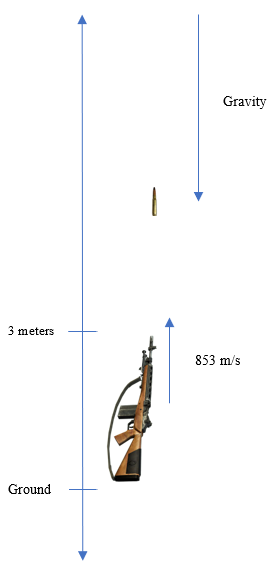
\includegraphics[height = 11cm]{Photos/Prob1Diagram.png}
			\end{figure}
			\newpage
			\item \textbf{Equations for the problem’s mathematical model:}
			\\ \\
			We can determine the position of the bullet by taking the product of the muzzle velocity with time and then subtracting the force of gravity and adding 3 meters because of its starting position:
			\[\boldsymbol{y(t) = vt - \frac{1}{2}gt^2 + 3}\]
			where $v = 853$ is the muzzle velocity, $g = 9.8$ is the constant of gravity, and $t$ represents the time in seconds after the bullet is shot. 
			\\
			\item \textbf{Solution of the model equations:}
			\\ \\
			Notice that the bullet reaches a maximum height when the velocity of the bullet, $\frac{dy}{dt} = 0$
			\begin{align*}
				\frac{dy}{dt} = v - gt &= 0 & t &= \frac{853}{9.8} \\
				853 - 9.8t &= 0 & &= 87.0408\,s
			\end{align*} 
			Now we can simply plug $\boldsymbol{t_{maxHeight} = 87.0408\,s}$ into our position function $y(t)$ to get the maximum height of $\boldsymbol{y_{max} = 37125.9082\,m}$
			\\ \\
			We can calculate when the bullet reaches the ground with the following equation:
			\begin{align*}
				y(t) = vt - \frac{1}{2}gt^2 + 3 &= 0 \\
				853t - \frac{1}{2}(9.8)t^2 + 3 &= 0 \\
				4.9t^2 - 853t - 3 &= 0
			\end{align*}
			We can now use the quadratic formula to solve for $t_{ground} > 0$:
			\begin{align*}
				t = \frac{853 \pm \sqrt{(-853)^2 - 4(4.9)(-3)}}{2(4.9)} = -.0035, 174.0851
			\end{align*}
			Thus we get that the bullet reaches the ground at $\boldsymbol{t_{ground} = 174.0851}$
			\newpage
\begin{Shaded}
\begin{Highlighting}[]
\CommentTok{# Problem 1 Model}

\NormalTok{v =}\StringTok{ }\DecValTok{853}
\NormalTok{g =}\StringTok{ }\FloatTok{9.8}
\NormalTok{t =}\StringTok{ }\KeywordTok{seq}\NormalTok{(}\OperatorTok{-}\DecValTok{25}\NormalTok{,}\DecValTok{200}\NormalTok{)}
\NormalTok{y =}\StringTok{ }\ControlFlowTok{function}\NormalTok{(t) v}\OperatorTok{*}\NormalTok{t }\OperatorTok{-}\StringTok{ }\NormalTok{(g}\OperatorTok{*}\NormalTok{t}\OperatorTok{^}\DecValTok{2} \OperatorTok{/}\StringTok{ }\DecValTok{2}\NormalTok{) }\OperatorTok{+}\StringTok{ }\DecValTok{3}
\NormalTok{ykm =}\StringTok{ }\ControlFlowTok{function}\NormalTok{(t) }\KeywordTok{y}\NormalTok{(t) }\OperatorTok{/}\StringTok{ }\DecValTok{1000}
\NormalTok{dy =}\StringTok{ }\ControlFlowTok{function}\NormalTok{(t) v }\OperatorTok{-}\StringTok{ }\NormalTok{g}\OperatorTok{*}\NormalTok{t}


\KeywordTok{plot}\NormalTok{(t, }\KeywordTok{ykm}\NormalTok{(t), }\StringTok{'l'}\NormalTok{, }\DataTypeTok{col=}\StringTok{'blue'}\NormalTok{, }
     \DataTypeTok{xlab =} \StringTok{'Time (sec)'}\NormalTok{, }\DataTypeTok{ylab =} \StringTok{'Height from the Ground (km)'}\NormalTok{, }
     \DataTypeTok{main =} \StringTok{'Height of Bullet from Ground over time'}\NormalTok{, }\DataTypeTok{panel.first=}\KeywordTok{grid}\NormalTok{())}
\KeywordTok{lines}\NormalTok{(t, }\DecValTok{0}\OperatorTok{*}\NormalTok{t, }\DataTypeTok{col=}\StringTok{'black'}\NormalTok{)}
\end{Highlighting}
\end{Shaded}

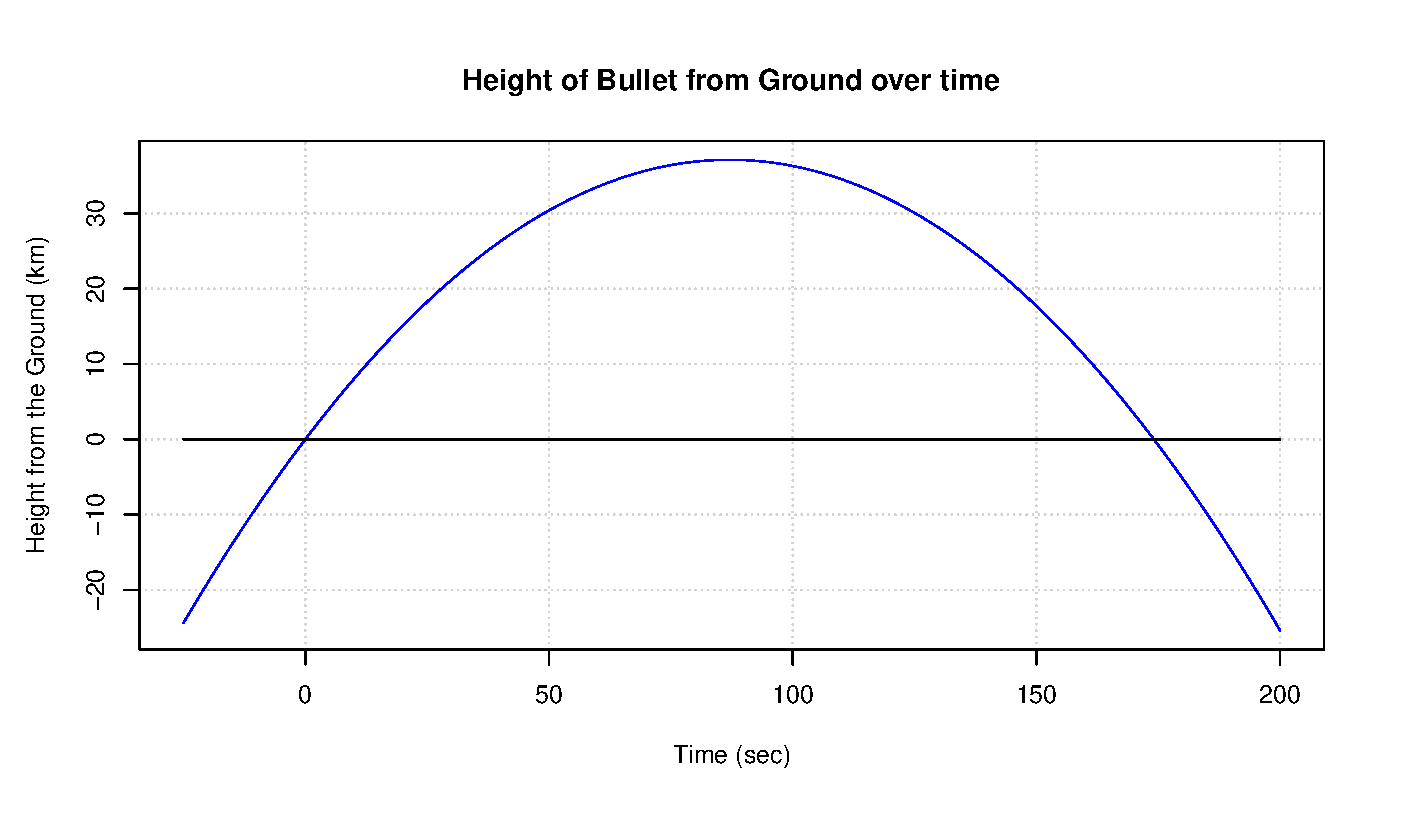
\includegraphics{Photos/Prob1}

\begin{Shaded}
\begin{Highlighting}[]
\KeywordTok{sprintf}\NormalTok{(}\StringTok{"Bullet Reaches Maximum Height at t = %.4f sec"}\NormalTok{, }
        \KeywordTok{uniroot}\NormalTok{(dy, }\KeywordTok{c}\NormalTok{(}\DecValTok{0}\NormalTok{,}\DecValTok{200}\NormalTok{))[[}\DecValTok{1}\NormalTok{]] )}
\end{Highlighting}
\end{Shaded}

\begin{verbatim}
## [1] "Bullet Reaches Maximum Height at t = 87.0408 sec"
\end{verbatim}

\begin{Shaded}
\begin{Highlighting}[]
\KeywordTok{sprintf}\NormalTok{(}\StringTok{"Bullet Reaches a Maximum Height of %.4f km"}\NormalTok{, }
        \KeywordTok{ykm}\NormalTok{(}\KeywordTok{uniroot}\NormalTok{(dy, }\KeywordTok{c}\NormalTok{(}\DecValTok{0}\NormalTok{,}\DecValTok{200}\NormalTok{))[[}\DecValTok{1}\NormalTok{]]))}
\end{Highlighting}
\end{Shaded}

\begin{verbatim}
## [1] "Bullet Reaches a Maximum Height of 37.1259 km"
\end{verbatim}

\begin{Shaded}
\begin{Highlighting}[]
\KeywordTok{sprintf}\NormalTok{(}\StringTok{"Bullet Touches the Ground at t = %.f sec"}\NormalTok{, }
        \KeywordTok{uniroot}\NormalTok{(ykm,}\KeywordTok{c}\NormalTok{(}\DecValTok{100}\NormalTok{,}\DecValTok{200}\NormalTok{))[}\DecValTok{1}\NormalTok{])}
\end{Highlighting}
\end{Shaded}

\begin{verbatim}
## [1] "Bullet Touches the Ground at t = 174 sec"
\end{verbatim}

			\newpage
			\item \textbf{Interpretation of the model solutions:}
			\\ \\
			When the M14 bullet is shot with a muzzle velocity of 853 m/s, it reaches its maximum height of 37.1259082 km, 87.0408 seconds after being shot.  It also returns to the ground 174.0851 seconds after being shot. 
			\\ \\
			The max height may change due to many factors such as weather, quality of the bullet, and conditions of the rifle.  So we must preform a sensitivity analysis, that is the sensitivity of the max height, $Y$ to the muzzle velocity, $v$.
			\[\Delta Y = S\Delta v, \qquad S = \frac{\Delta Y}{\Delta v} = \frac{dY}{dv}\]
			where S is called the sensitivity factor or relative sensitivity.
			\\ \\
			So thus we get the following:
			\begin{align*}
				y\left(\frac{v}{g}\right) = Y(v) &= v\left(\frac{v}{g}\right) - \frac{1}{2}g\left(\frac{v}{g}\right)^2 + 3 = \frac{v^2}{2g} + 3 \\
				\frac{dY}{dv} &= \frac{v}{g}
			\end{align*}
			\begin{figure}[h!]
				\centering
				\begin{tabular}{|c|c|c|c|}
					\hline
					$v$ & \% from 853 & SY & \% from 87.041 \\
					\hline
					813 & -4.6893 \%  & 82.9592 & -4.6893 \% \\  
					833 & -2.3447 \%  & 85.0000 & -2.3447 \% \\
					853 & 0.0000  \%  & 87.0408 & 0.0000  \%\\
					873 & 2.3447 \%   & 89.0816 & 2.3447 \% \\
					893 & 4.6893 \%   & 91.1224 & 4.6893 \% \\
					\hline
				\end{tabular}
			\end{figure}  
			\\ 
			Notice that per every 20 meters in initial velocity, the max height changes by about 2 meters. Or for every 2.3\% change in initial velocity, there is a 2.3\% change in max height.  This makes sense because $\Delta S = v / g$ means that the sensitivity is directly proportional to its velocity, $v$.
			\newpage
\begin{Shaded}
\begin{Highlighting}[]
\NormalTok{x =}\StringTok{ }\DecValTok{1}
\NormalTok{v =}\StringTok{ }\KeywordTok{seq}\NormalTok{(}\DecValTok{813}\NormalTok{,}\DecValTok{893}\NormalTok{, }\DataTypeTok{by =} \DecValTok{20}\NormalTok{)}
\NormalTok{SY =}\StringTok{ }\KeywordTok{seq}\NormalTok{(}\DecValTok{1}\NormalTok{, }\KeywordTok{length}\NormalTok{(v))}
\NormalTok{perChange583 =}\StringTok{ }\KeywordTok{seq}\NormalTok{(}\DecValTok{1}\NormalTok{, }\KeywordTok{length}\NormalTok{(v))}
\NormalTok{perChange87 =}\StringTok{ }\KeywordTok{seq}\NormalTok{(}\DecValTok{1}\NormalTok{, }\KeywordTok{length}\NormalTok{(v))}
\ControlFlowTok{for}\NormalTok{ (val }\ControlFlowTok{in}\NormalTok{ v) \{}
\NormalTok{  perChange583[x] =}\StringTok{ }\KeywordTok{round}\NormalTok{( (val }\OperatorTok{-}\StringTok{ }\DecValTok{853}\NormalTok{) }\OperatorTok{*}\StringTok{ }\DecValTok{100} \OperatorTok{/}\StringTok{ }\DecValTok{853}\NormalTok{, }\DataTypeTok{digits =} \DecValTok{4}\NormalTok{) }
\NormalTok{  SY[x] =}\StringTok{ }\KeywordTok{round}\NormalTok{( val }\OperatorTok{/}\StringTok{ }\FloatTok{9.8}\NormalTok{ , }\DataTypeTok{digits =} \DecValTok{4}\NormalTok{ )}
\NormalTok{  perChange87[x] =}\StringTok{ }\KeywordTok{round}\NormalTok{( (SY[x] }\OperatorTok{-}\StringTok{ }\NormalTok{(}\DecValTok{853} \OperatorTok{/}\StringTok{ }\FloatTok{9.8}\NormalTok{)) }\OperatorTok{*}\StringTok{ }\DecValTok{100} \OperatorTok{/}\StringTok{ }\NormalTok{(}\DecValTok{853} \OperatorTok{/}\StringTok{ }\FloatTok{9.8}\NormalTok{), }\DataTypeTok{digits =} \DecValTok{4}\NormalTok{) }
\NormalTok{  x =}\StringTok{ }\NormalTok{x }\OperatorTok{+}\StringTok{ }\DecValTok{1}
\NormalTok{\}}

\NormalTok{table =}\StringTok{ }\KeywordTok{cbind}\NormalTok{(v, perChange583, SY, perChange87)}
\KeywordTok{colnames}\NormalTok{(table) =}\StringTok{ }\KeywordTok{c}\NormalTok{(}\StringTok{'v'}\NormalTok{, }\StringTok{'% from 583'}\NormalTok{, }\StringTok{'SY'}\NormalTok{, }\StringTok{'% from 87.041'}\NormalTok{)}
\NormalTok{table}
\end{Highlighting}
\end{Shaded}

\begin{verbatim}
##        v % from 583      SY % from 87.041
## [1,] 813    -4.6893 82.9592       -4.6893
## [2,] 833    -2.3447 85.0000       -2.3447
## [3,] 853     0.0000 87.0408        0.0000
## [4,] 873     2.3447 89.0816        2.3446
## [5,] 893     4.6893 91.1224        4.6893
\end{verbatim}
		
		\end{enumerate}
	\end{problem}


	\begin{problem}{2 Exercise (4.6)}
		A more complex annuity payment calculation: You would like to put away some
		money every month for your retirement when you reach 30 years old. You plan to retire at
		age of 68 and live up to 118 years old. You would like to be able to draw \$1,000 per month,
		called annuity payment, from the saving from the first month of your 69th year, i.e., the
		first month after your 68th birthday. The money is all used up when you reach your 118th
		birthday. If the annuity interest rate is 5\% per year, how much you need to start paying to
		your annuity fund when you reach 30 until your retirement? You can use a method similar
		to the mortgage calculation.
		\\ \\
		From his 30th birthday to his 68th birthday, he is accruing interest and actively putting in a monthly payment, $x$, into his retirement account.  From his 68th birthday to his 118th birthday, he is accruing interest and taking out $\$1,000$ a month from his retirement account with $P$ dollars initially, the amount of money he accrued from his 30th birthday to his 68th.
		\\ \\
		Notice the following with $M_i$ being the amount of money he has per month in his retirement and $i = 1,2...$  
		\begin{align*}
			M_1 &= P(1+r) - 1000 \\
			M_2 &= P(1+r)^2 - 1000(1+r) - 1000
		\end{align*}
		So notice the following for a general case, $k$:
		\begin{align*}
			M_k &= P(1+r)^k - 1000\left((1+r)^{k-1} + \cdots + (1+r) + 1 \right) \\
			&= P(1+r)^k - 1000\left( \frac{1 - (1 + r)^k}{1 - (1 + r)} \right) 
		\end{align*}
		When he turns 118, that would be 600 months from his 68th birthday, he should have 0 dollars in his retirement account so we let $M_{k = 600} = 0$ and $r = .05 / 12$
		\begin{align*}
			M_{600} = 0 &= P\left(1 + \frac{.05}{12}\right)^{600} - 1000\left( \frac{1 - (1 + (.05 / 12))^{600}}{1 - (1 + (.05 / 12))} \right) \\
			&= P\left(12.1194\right) - 2668651.971 
		\end{align*}
		Using some simple algebra now, we get that:
		\[\boldsymbol{P = \$220,197.01}\]
		What $P$ represents is the amount of money he need to accrue from his 30th birthday to his 68th birthday.

\begin{Shaded}
\begin{Highlighting}[]
\CommentTok{# Problem 2}

\NormalTok{k =}\StringTok{ }\DecValTok{600}
\NormalTok{r =}\StringTok{ }\FloatTok{.05} \OperatorTok{/}\StringTok{ }\DecValTok{12}
\NormalTok{y =}\StringTok{ }\DecValTok{1000}

\NormalTok{M =}\StringTok{ }\ControlFlowTok{function}\NormalTok{(P) \{}
\NormalTok{  P }\OperatorTok{*}\StringTok{ }\NormalTok{((}\DecValTok{1} \OperatorTok{+}\StringTok{ }\NormalTok{r)}\OperatorTok{^}\NormalTok{k) }\OperatorTok{-}\StringTok{ }\NormalTok{y}\OperatorTok{*}\NormalTok{( (}\DecValTok{1} \OperatorTok{-}\StringTok{ }\NormalTok{(}\DecValTok{1} \OperatorTok{+}\StringTok{ }\NormalTok{r)}\OperatorTok{^}\NormalTok{k) }\OperatorTok{/}\StringTok{ }\NormalTok{(}\DecValTok{1} \OperatorTok{-}\StringTok{ }\NormalTok{(}\DecValTok{1} \OperatorTok{+}\StringTok{ }\NormalTok{r)) )}
\NormalTok{\}}
\NormalTok{P =}\StringTok{ }\KeywordTok{uniroot}\NormalTok{(M,}\KeywordTok{c}\NormalTok{(}\DecValTok{200000}\NormalTok{,}\DecValTok{300000}\NormalTok{))[[}\DecValTok{1}\NormalTok{]]}
\KeywordTok{sprintf}\NormalTok{(}\StringTok{'By the Age of 68, He will need P = $%.02f in his Retirement Account'}\NormalTok{,P)}
\end{Highlighting}
\end{Shaded}

\begin{verbatim}
## [1] "By the Age of 68, He will need P = $220197.01 in his Retirement Account"
\end{verbatim}

		\newpage
		Now notice the following with $N_i$ being the amount of money he has per month while working with $i = 1,2...$.
		\begin{align*}
			N_1 &= x \\
			N_2 &= x(1+r) + x \\
			N_3 &= x(1+r)^2 + x(1+r) + x
		\end{align*}
		So notice the following for a general case, $k$:
		\begin{align*}
			N_k &= x\left((1+r)^{k-1} + \cdots + (1+r) + 1 \right) = x\left(\frac{1 - (1+r)^{k}}{1 - (1+r)}\right)
		\end{align*}
		When he turns 68, that would be 456 months from his 30th birthday, he should have $P = 22,0197.01$ dollars in his retirement account, so we let $N_{456} = 220197.01$ and $r = .05/12$.
		\begin{align*}
			N_{456} = 220197.01 &= x\left(\frac{1 - (1+(.05/12))^{456}}{1 - (1+(.05/12))}\right) \\
			&= 1358.29314x
		\end{align*} 
		Using some simple algebra, we get that the monthly payment will be:
		\[\boldsymbol{x = \$162.11}\]
	
\begin{Shaded}
\begin{Highlighting}[]
\NormalTok{k =}\StringTok{ }\DecValTok{456}
\NormalTok{N =}\StringTok{ }\ControlFlowTok{function}\NormalTok{(x) \{}
\NormalTok{  x }\OperatorTok{*}\StringTok{ }\NormalTok{( (}\DecValTok{1} \OperatorTok{-}\StringTok{ }\NormalTok{(}\DecValTok{1} \OperatorTok{+}\StringTok{ }\NormalTok{r)}\OperatorTok{^}\NormalTok{k) }\OperatorTok{/}\StringTok{ }\NormalTok{(}\DecValTok{1} \OperatorTok{-}\StringTok{ }\NormalTok{(}\DecValTok{1} \OperatorTok{+}\StringTok{ }\NormalTok{r)) ) }\OperatorTok{-}\StringTok{ }\NormalTok{P}
\NormalTok{\}}
\NormalTok{x =}\StringTok{ }\KeywordTok{uniroot}\NormalTok{(N, }\KeywordTok{c}\NormalTok{(}\DecValTok{0}\NormalTok{,}\DecValTok{1000}\NormalTok{))[[}\DecValTok{1}\NormalTok{]]}
\KeywordTok{sprintf}\NormalTok{(}\StringTok{'He will need to pay $%.02f a month to retire correctly'}\NormalTok{,x)}
\end{Highlighting}
\end{Shaded}

\begin{verbatim}
## [1] "He will need to pay $162.11 a month to retire correctly"
\end{verbatim}

	\end{problem}
	
	
	\begin{problem}{3 Exercise (4.7)}
		Use the EBM and R to estimate the lunar surface temperature at lunar latitude $30^{\circ}$
		North and at 3:00 PM, lunar local time. Hint: The 12:00 PM noon for a lunar location is
		when the location directly faces the Sun. From this point, the location of 3:00 PM can be
		found.
		\\ \\
		We have the following: 
		\begin{itemize}[label = -]
			\item So we get the solar constant of $S = 1368$ $W/m^2$ (Solar constant of the moon is the same as Earth's due to their distance to the sun).
			\item The moon has an average albedo value of about $\alpha = 0.12$.
			\item The thermal conductivity of the moon’s surface regolith $\kappa = 7.4 \times 10^-4$ $[Wm^{-1} / K^\circ ]$.
			\item The deep crusts temperature to be at a constant $T_0 = 260 K$.
			\item $h = 0.4$,  which is the lunar crust’s depth that can be reached by the thermal conduction from the surface
			\item $\sigma = 5.670367 \times 10^{-8} $ $[Wm^{-2}K^{-4}]$ is the Stefan-Boltzmann constant. 
			\item $\epsilon = 0.98$ is the lunar surface’s emissivity
		\end{itemize}
		To find the surface temperature with respect to the lunar latitude, $\beta$, we use the following equation:
		\[(1 - \alpha)S\cos\beta\cos\theta = \epsilon\sigma T^{4} + \kappa \frac{T - T_0}{h}\]
		Using R code to solve for the temperature, we get the following:
		\\ \\
		Notice that if noon is $0^\circ$ longitude and if midnight is $180^\circ$ longitude, then 3:00pm would be $45^\circ$ longitude. Thus we get the following:
		\\ \\
		The Lunar Surface Temperature of the Moon at 30.00 degrees latitude and 45.00 degrees longitude is \textbf{339.3635 K}.
		\newpage
\begin{Shaded}
\begin{Highlighting}[]
\CommentTok{# Problem 3}

\NormalTok{EBM =}\StringTok{ }\ControlFlowTok{function}\NormalTok{(beta, theta) \{}
\NormalTok{  lat =}\StringTok{ }\NormalTok{beta }\OperatorTok{*}\StringTok{ }\NormalTok{pi }\OperatorTok{/}\StringTok{ }\DecValTok{180}
\NormalTok{  lon =}\StringTok{ }\NormalTok{theta }\OperatorTok{*}\StringTok{ }\NormalTok{pi }\OperatorTok{/}\StringTok{ }\DecValTok{180}
\NormalTok{  S =}\StringTok{ }\DecValTok{1368}
\NormalTok{  alpha =}\StringTok{ }\FloatTok{0.12}
\NormalTok{  k =}\StringTok{ }\FloatTok{7.4} \OperatorTok{*}\StringTok{ }\DecValTok{10}\OperatorTok{^}\NormalTok{(}\OperatorTok{-}\DecValTok{4}\NormalTok{)}
\NormalTok{  T0 =}\StringTok{ }\DecValTok{260}
\NormalTok{  h =}\StringTok{ }\FloatTok{0.4}
\NormalTok{  sigma =}\StringTok{ }\FloatTok{5.670367}\OperatorTok{*}\DecValTok{10}\OperatorTok{^}\NormalTok{(}\OperatorTok{-}\DecValTok{8}\NormalTok{)}
\NormalTok{  ep =}\StringTok{ }\FloatTok{0.98}

\NormalTok{  fEBM =}\StringTok{ }\ControlFlowTok{function}\NormalTok{(T) \{ (}\DecValTok{1} \OperatorTok{-}\StringTok{ }\NormalTok{alpha) }\OperatorTok{*}\StringTok{ }\NormalTok{S }\OperatorTok{*}\StringTok{ }\KeywordTok{cos}\NormalTok{(lat) }\OperatorTok{*}\StringTok{ }\KeywordTok{cos}\NormalTok{(lon) }\OperatorTok{-}\StringTok{ }
\StringTok{                       }\NormalTok{( ep }\OperatorTok{*}\StringTok{ }\NormalTok{sigma }\OperatorTok{*}\StringTok{ }\NormalTok{T}\OperatorTok{^}\DecValTok{4} \OperatorTok{+}\StringTok{ }\NormalTok{k }\OperatorTok{*}\StringTok{ }\NormalTok{(T }\OperatorTok{-}\StringTok{ }\NormalTok{T0) }\OperatorTok{/}\StringTok{ }\NormalTok{h ) \}}

  \KeywordTok{sprintf}\NormalTok{(}\StringTok{"The Lunar Surface Temperature of the Moon at }
          \StringTok{%.2f degrees latitude and %.2f degrees longitude is %.4f K"}\NormalTok{,}
\NormalTok{          beta, theta, }\KeywordTok{uniroot}\NormalTok{(fEBM,}\KeywordTok{c}\NormalTok{(}\DecValTok{100}\NormalTok{,}\DecValTok{420}\NormalTok{))[[}\DecValTok{1}\NormalTok{]])}
\NormalTok{\}}

\KeywordTok{EBM}\NormalTok{(}\DecValTok{30}\NormalTok{, }\DecValTok{45}\NormalTok{)}
\end{Highlighting}
\end{Shaded}

\begin{verbatim}
## [1] "The Lunar Surface Temperature of the Moon at 30.00 degrees latitude 
        and 45.00 degrees longitude is 339.3635 K"
\end{verbatim}
	
	\end{problem}


	\begin{problem}{4 Exercise (4.8)}
		Use the EBM and R to estimate the lunar surface temperature at 24 points uniformly
		distributed on the equator. List the results in a table of three columns. The first column is
		longitude, the second is temperature in Kelvin, and third is temperature in degrees Celsius.
		\\ \\
		\begin{figure}[h!]
			\centering
			\begin{tabular}{|c|c|c|}
				\hline
				Longitude & Temp (K) & Temp ($^\circ C$) \\
				\hline
 				 0 & 383.62972 & 110.6297190 \\
			    15 & 380.31901 &  107.3190064 \\
			    30 & 370.07888 &   97.0788846 \\
			    45 & 351.78919 &   78.7891881 \\
			    60 & 322.59265 &  49.5926535 \\
			    75 & 273.63595 &  0.6359485 \\
			    90 &  51.33862 & -221.6613844 \\
			   105 & 101.37564 & -171.6243637 \\
			   120 & 101.37564 & -171.6243637 \\
			   135 & 101.37564 & -171.6243637 \\
			   150 & 101.37564 & -171.6243637 \\
			   165 & 101.37564 & -171.6243637 \\
			   180 & 101.37564 & -171.6243637 \\
			   195 & 101.37564 & -171.6243637 \\
			   210 & 101.37564 & -171.6243637 \\
			   225 & 101.37564 & -171.6243637 \\
			   240 & 101.37564 & -171.6243637 \\
			   255 & 101.37564 & -171.6243637 \\
			   270 &  51.33862 & -221.6613844 \\
			   285 & 273.63595 &    0.6359485 \\ 
			   300 & 322.59265 &   49.5926535 \\
			   315 & 351.78919 &   78.7891881 \\
			   330 & 370.07888 &   97.0788846 \\ 
			   345 & 380.31901 &  107.3190064 \\
			   \hline
			\end{tabular}
		\end{figure}
		\\ \\
		Notice for $90 < \theta < 270$, we get a constant temperature of $101.37564$ K.  This is because within that angle range, that side of the moon does not receive any solar radiation to heat up the surface.
		\newpage
\begin{Shaded}
\begin{Highlighting}[]
\CommentTok{# Problem 4}

\NormalTok{EBM =}\StringTok{ }\ControlFlowTok{function}\NormalTok{(theta) \{}
\NormalTok{  lat =}\StringTok{ }\DecValTok{0}
\NormalTok{  lon =}\StringTok{ }\NormalTok{theta }\OperatorTok{*}\StringTok{ }\NormalTok{pi }\OperatorTok{/}\StringTok{ }\DecValTok{180}
\NormalTok{  alpha =}\StringTok{ }\FloatTok{0.12}
\NormalTok{  k =}\StringTok{ }\FloatTok{7.4} \OperatorTok{*}\StringTok{ }\DecValTok{10}\OperatorTok{^}\NormalTok{(}\OperatorTok{-}\DecValTok{4}\NormalTok{)}
\NormalTok{  T0 =}\StringTok{ }\DecValTok{260}
\NormalTok{  sigma =}\StringTok{ }\FloatTok{5.670367}\OperatorTok{*}\DecValTok{10}\OperatorTok{^}\NormalTok{(}\OperatorTok{-}\DecValTok{8}\NormalTok{)}
\NormalTok{  ep =}\StringTok{ }\FloatTok{0.98}
\NormalTok{  h =}\StringTok{ }\FloatTok{0.4}
\NormalTok{  S =}\StringTok{ }\DecValTok{1368}
  \ControlFlowTok{if}\NormalTok{ (theta }\OperatorTok{>}\StringTok{ }\DecValTok{90} \OperatorTok{&&}\StringTok{ }\NormalTok{theta }\OperatorTok{<}\StringTok{ }\DecValTok{270}\NormalTok{ ) \{}
\NormalTok{    h =}\StringTok{ }\FloatTok{0.02}
\NormalTok{    S =}\StringTok{ }\DecValTok{0}
\NormalTok{  \}}

\NormalTok{  fEBM =}\StringTok{ }\ControlFlowTok{function}\NormalTok{(T) \{ (}\DecValTok{1} \OperatorTok{-}\StringTok{ }\NormalTok{alpha) }\OperatorTok{*}\StringTok{ }\NormalTok{S }\OperatorTok{*}\StringTok{ }\KeywordTok{cos}\NormalTok{(lat) }\OperatorTok{*}\StringTok{ }\KeywordTok{cos}\NormalTok{(lon) }\OperatorTok{-}\StringTok{ }
\StringTok{                     }\NormalTok{(ep }\OperatorTok{*}\StringTok{ }\NormalTok{sigma }\OperatorTok{*}\StringTok{ }\NormalTok{T}\OperatorTok{^}\DecValTok{4} \OperatorTok{+}\StringTok{ }\NormalTok{k }\OperatorTok{*}\StringTok{ }\NormalTok{(T }\OperatorTok{-}\StringTok{ }\NormalTok{T0) }\OperatorTok{/}\StringTok{ }\NormalTok{h ) \}}

  \KeywordTok{sprintf}\NormalTok{(}\StringTok{"The Lunar Surface Temperature of the Moon at %.2f degrees is %.4f K"}\NormalTok{, }
\NormalTok{          theta, }\KeywordTok{uniroot}\NormalTok{(fEBM,}\KeywordTok{c}\NormalTok{(}\DecValTok{0}\NormalTok{,}\DecValTok{500}\NormalTok{))[[}\DecValTok{1}\NormalTok{]])}

  \KeywordTok{return}\NormalTok{(}\KeywordTok{uniroot}\NormalTok{(fEBM,}\KeywordTok{c}\NormalTok{(}\DecValTok{0}\NormalTok{,}\DecValTok{500}\NormalTok{))[[}\DecValTok{1}\NormalTok{]])}
\NormalTok{\}}
\end{Highlighting}
\end{Shaded}
\newpage
\begin{Shaded}
\begin{Highlighting}
\NormalTok{x =}\StringTok{ }\DecValTok{1}
\NormalTok{longitude =}\StringTok{ }\KeywordTok{matrix}\NormalTok{(}\KeywordTok{seq}\NormalTok{(}\DecValTok{0}\NormalTok{,}\DecValTok{359}\NormalTok{,}\DataTypeTok{by=}\DecValTok{15}\NormalTok{),}\DataTypeTok{ncol=}\DecValTok{1}\NormalTok{)}
\NormalTok{Ktemp =}\StringTok{ }\KeywordTok{matrix}\NormalTok{(}\KeywordTok{seq}\NormalTok{(}\DecValTok{1}\NormalTok{, }\KeywordTok{length}\NormalTok{(longitude)), }\DataTypeTok{ncol =} \DecValTok{1}\NormalTok{)}
\NormalTok{Ctemp =}\StringTok{ }\KeywordTok{matrix}\NormalTok{(}\KeywordTok{seq}\NormalTok{(}\DecValTok{1}\NormalTok{, }\KeywordTok{length}\NormalTok{(longitude)), }\DataTypeTok{ncol =} \DecValTok{1}\NormalTok{)}
\ControlFlowTok{for}\NormalTok{ (i }\ControlFlowTok{in}\NormalTok{ longitude) \{}
\NormalTok{  Ktemp[x] =}\StringTok{ }\KeywordTok{EBM}\NormalTok{(i)}
\NormalTok{  Ctemp[x] =}\StringTok{ }\NormalTok{Ktemp[x] }\OperatorTok{-}\StringTok{ }\DecValTok{273}
\NormalTok{  x =}\StringTok{ }\NormalTok{x }\OperatorTok{+}\StringTok{ }\DecValTok{1}
\NormalTok{\}}

\NormalTok{table =}\StringTok{ }\KeywordTok{cbind}\NormalTok{(longitude, Ktemp, Ctemp)}
\KeywordTok{colnames}\NormalTok{(table) =}\StringTok{ }\KeywordTok{c}\NormalTok{(}\StringTok{'Long'}\NormalTok{, }\StringTok{'Temp (K)'}\NormalTok{, }\StringTok{'Temp (C)'}\NormalTok{)}
\NormalTok{table}
\end{Highlighting}
\end{Shaded}

\begin{verbatim}
##       Long  Temp (K)     Temp (C)
##  [1,]    0 383.62972  110.6297190
##  [2,]   15 380.31901  107.3190064
##  [3,]   30 370.07888   97.0788846
##  [4,]   45 351.78919   78.7891881
##  [5,]   60 322.59265   49.5926535
##  [6,]   75 273.63595    0.6359485
##  [7,]   90  51.33862 -221.6613844
##  [8,]  105 101.37564 -171.6243637
##  [9,]  120 101.37564 -171.6243637
## [10,]  135 101.37564 -171.6243637
## [11,]  150 101.37564 -171.6243637
## [12,]  165 101.37564 -171.6243637
## [13,]  180 101.37564 -171.6243637
## [14,]  195 101.37564 -171.6243637
## [15,]  210 101.37564 -171.6243637
## [16,]  225 101.37564 -171.6243637
## [17,]  240 101.37564 -171.6243637
## [18,]  255 101.37564 -171.6243637
## [19,]  270  51.33862 -221.6613844
## [20,]  285 273.63595    0.6359485
## [21,]  300 322.59265   49.5926535
## [22,]  315 351.78919   78.7891881
## [23,]  330 370.07888   97.0788846
## [24,]  345 380.31901  107.3190064
\end{verbatim}
			
	\end{problem}


	\begin{problem}{5 Exercise (4.11)}
		EBM sensitivity analysis for emissivity.
		\begin{enumerate}[label = (\alph*)]
			\item Following the sensitivity analysis method at the end of the section on zeroing a
			rifle, make a sensitivity analysis for the simple zero-dimensional energy balance
			climate model with respect to emissivity $\epsilon$ around 0.6. The EBM model equation
			is below
			\[(1-\alpha)S/4 = \epsilon \sigma T^4\]
			Use a table to document how the Earth temperature vary with respect to the perturbation of $\epsilon$. Here, the Earth reflectivity is assumed to be fixed at $\alpha = 0.32$, and the Stefan-Boltzmann constant is $\sigma = 5.670373 \times 10^{-8}\,[Wm^{-2}K^{-4}] $
			\\ \\
			Notice we can find the sensitivity analysis from the following equation:
			\[\Delta T = S \Delta \epsilon, \qquad S = \frac{\Delta T}{\Delta \epsilon} = \frac{dT}{d\epsilon}\]
			\begin{align*}
				T = \sqrt[4]{\frac{S}{4\sigma}\left(1 - \alpha \right)}\,\epsilon^{-1/4} &&
				\frac{dT}{d\epsilon} = \frac{-1}{4}\sqrt[4]{\frac{S}{4\sigma}\left(1 - \alpha \right)}\,\epsilon^{-5/4}
			\end{align*}
			\\ 
			\begin{figure}[h!]
				\centering
				\begin{tabular}{|c|c|c|c|}
					\hline
					$\epsilon$ & \% from .60 & ST & \% from -119.8069\\
					\hline
					0.55  &  -8.3333 \%  &   -133.5727  &   11.4899 \% \\
					0.56  &  -6.6667 \%  &   -130.5978  &   9.0069 \% \\
					0.57  &  -5.0000 \%  &   -127.7401  &   6.6217 \% \\
					0.58  &  -3.3333 \%  &   -124.9931  &   4.3288 \% \\
					0.59  &  -1.6667 \%  &   -122.3506  &   2.1231 \% \\
					0.60  &   0.0000 \%  &   -119.8069  &   0.0000 \% \\
					0.61  &   1.6667 \%  &   -117.3569  &   -2.0450 \% \\
					0.62  &   3.3333 \%  &   -114.9956  &   -4.0159 \% \\
					0.63  &   5.0000 \%  &   -112.7185  &   -5.9165 \% \\
					0.64  &   6.6667 \%  &   -110.5213  &   -7.7505 \% \\
					0.65  &   8.3333 \%  &   -108.4000  &   -9.5211 \% \\
					\hline		
				\end{tabular}
			\end{figure}
			\newpage 

\begin{Shaded}
\begin{Highlighting}[]
\CommentTok{# Problem 5}

\NormalTok{x =}\StringTok{ }\DecValTok{1}
\NormalTok{Ep =}\StringTok{ }\KeywordTok{matrix}\NormalTok{(}\KeywordTok{seq}\NormalTok{(.}\DecValTok{55}\NormalTok{, }\FloatTok{.65}\NormalTok{, }\DataTypeTok{by=}\NormalTok{.}\DecValTok{01}\NormalTok{), }\DataTypeTok{ncol =} \DecValTok{1}\NormalTok{)}
\NormalTok{perChange60 =}\StringTok{ }\KeywordTok{matrix}\NormalTok{(}\KeywordTok{seq}\NormalTok{(}\DecValTok{0}\NormalTok{,}\DecValTok{10}\NormalTok{), }\DataTypeTok{ncol =} \DecValTok{1}\NormalTok{)}
\NormalTok{ST =}\StringTok{ }\KeywordTok{matrix}\NormalTok{(}\KeywordTok{seq}\NormalTok{(}\DecValTok{0}\NormalTok{,}\DecValTok{10}\NormalTok{), }\DataTypeTok{ncol =} \DecValTok{1}\NormalTok{)}
\NormalTok{perChange119 =}\StringTok{ }\KeywordTok{matrix}\NormalTok{(}\KeywordTok{seq}\NormalTok{(}\DecValTok{0}\NormalTok{,}\DecValTok{10}\NormalTok{), }\DataTypeTok{ncol =} \DecValTok{1}\NormalTok{)}

\NormalTok{sigma =}\StringTok{ }\FloatTok{5.670367}\OperatorTok{*}\DecValTok{10}\OperatorTok{^}\NormalTok{(}\OperatorTok{-}\DecValTok{8}\NormalTok{)}
\NormalTok{S =}\StringTok{ }\DecValTok{1368}
\NormalTok{alpha =}\StringTok{ }\FloatTok{0.32}

\ControlFlowTok{for}\NormalTok{ (val }\ControlFlowTok{in}\NormalTok{ Ep)\{}
\NormalTok{  dT =}\StringTok{ }\ControlFlowTok{function}\NormalTok{(val) \{ (}\OperatorTok{-}\DecValTok{1}\OperatorTok{/}\DecValTok{4}\NormalTok{) }\OperatorTok{*}\StringTok{ }\NormalTok{(( (S }\OperatorTok{/}\StringTok{ }\NormalTok{(}\DecValTok{4} \OperatorTok{*}\StringTok{ }\NormalTok{sigma) ) }\OperatorTok{*}\StringTok{ }\NormalTok{(}\DecValTok{1} \OperatorTok{-}\StringTok{ }\NormalTok{alpha) )}\OperatorTok{^}\NormalTok{(}\DecValTok{1}\OperatorTok{/}\DecValTok{4}\NormalTok{)) }\OperatorTok{*}\StringTok{ }\NormalTok{((val)}\OperatorTok{^}\NormalTok{(}\OperatorTok{-}\DecValTok{5}\OperatorTok{/}\DecValTok{4}\NormalTok{)) \}}

\NormalTok{  perChange60[x] =}\StringTok{ }\KeywordTok{round}\NormalTok{(( val }\OperatorTok{-}\StringTok{ }\FloatTok{.60}\NormalTok{ ) }\OperatorTok{*}\StringTok{ }\DecValTok{100} \OperatorTok{/}\StringTok{ }\FloatTok{.60}\NormalTok{, }\DataTypeTok{digits =} \DecValTok{4}\NormalTok{) }
\NormalTok{  ST[x] =}\StringTok{ }\KeywordTok{dT}\NormalTok{(val)}
\NormalTok{  perChange119[x] =}\StringTok{ }\KeywordTok{round}\NormalTok{(( ST[x] }\OperatorTok{-}\StringTok{ }\KeywordTok{dT}\NormalTok{(.}\DecValTok{60}\NormalTok{) ) }\OperatorTok{*}\StringTok{ }\DecValTok{100} \OperatorTok{/}\StringTok{ }\KeywordTok{dT}\NormalTok{(.}\DecValTok{60}\NormalTok{), }
\DataTypeTok{digits =} \DecValTok{4}\NormalTok{  ) }
\NormalTok{  x =}\StringTok{ }\NormalTok{x }\OperatorTok{+}\StringTok{ }\DecValTok{1}
\NormalTok{\}}

\NormalTok{table =}\StringTok{ }\KeywordTok{cbind}\NormalTok{(Ep, perChange60, ST, perChange119)}
\KeywordTok{colnames}\NormalTok{(table) =}\StringTok{ }\KeywordTok{c}\NormalTok{(}\StringTok{'Epsilon'}\NormalTok{, }\StringTok{'% from .60'}\NormalTok{, }\StringTok{'ST'}\NormalTok{, }\StringTok{'% from ST(.60)'}\NormalTok{)}
\NormalTok{table}
\end{Highlighting}
\end{Shaded}

\begin{verbatim}
##       Epsilon % from .60        ST % from ST(.60)
##  [1,]    0.55    -8.3333 -133.5727        11.4899
##  [2,]    0.56    -6.6667 -130.5978         9.0069
##  [3,]    0.57    -5.0000 -127.7401         6.6217
##  [4,]    0.58    -3.3333 -124.9931         4.3288
##  [5,]    0.59    -1.6667 -122.3506         2.1231
##  [6,]    0.60     0.0000 -119.8069         0.0000
##  [7,]    0.61     1.6667 -117.3569        -2.0450
##  [8,]    0.62     3.3333 -114.9956        -4.0159
##  [9,]    0.63     5.0000 -112.7185        -5.9165
## [10,]    0.64     6.6667 -110.5213        -7.7505
## [11,]    0.65     8.3333 -108.4000        -9.5211
\end{verbatim}

			\newpage	
			\item Use 100-200 words to discuss the physical meaning of your numerical results
			from the perspectives of greenhouse gases and insulation.
			\\ \\
			Heat is trapped due to the greenhouse gases and insulation.  Because of this, the earth's temperature is actually hotter than our above model.  Our model would work if the earth consisted fully of water.  This is because we used the parameter that $\epsilon = 0.60$.  This doesn't take in account that the earth doesn't have an emissivity level of $\epsilon = 0.60$ uniformly around the globe.  We use that $\epsilon$ value because the earth consists of mostly water, however, "mostly" doesn't account for everything. We can see that for a $0.01$ change in $\epsilon$, we get about 2\% change in temperature.
		\end{enumerate}
	\end{problem}


	\begin{problem}{6 Exercise (5.1)}
		Solve an electric circuit shown in Fig. 5.7
		\begin{figure}[h!]
			\centering
			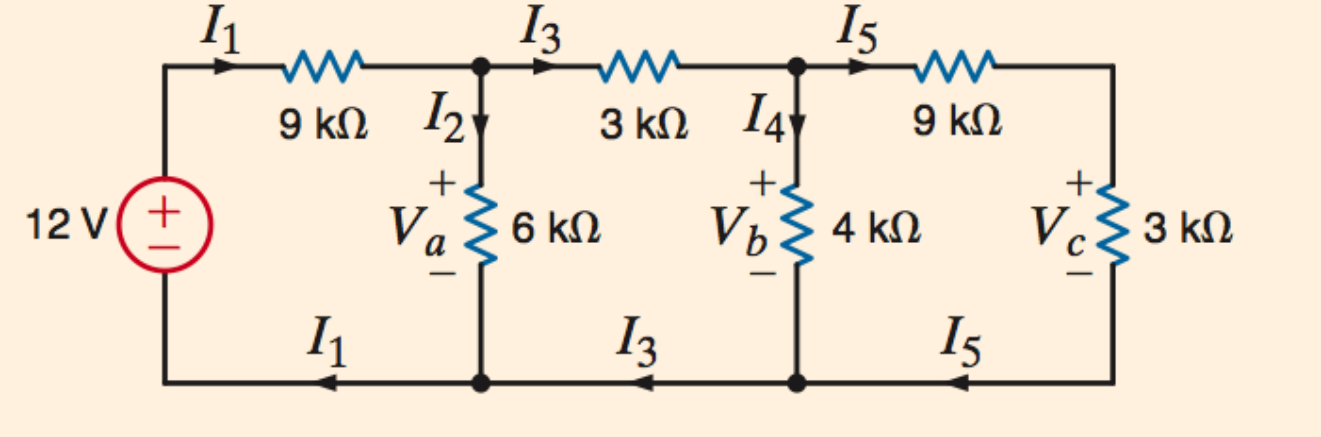
\includegraphics[width = 12cm]{Photos/Fig57.png}
			\captionsetup{labelformat=empty}
			\caption{\textbf{Figure 5.7} An electric circuit of one battery, six resistors and five currents. Notice that the bottom
				middle section’s current is also $I_3$ because any current from the top middle section has only one
				way to go back to the battery, and both the top-mid and bottom-mid sections have the same current
				$I_4$ + $I_5$.}
		\end{figure}
		\begin{enumerate}[label = (\alph*)]
			\item Find all the currents $I_1, I_2, I_3, I_4, I_5$.  [Hint: Use Kirchhoff’s law to set up five linear
			equations with $I_1, I_2, I_3, I_4, I_5$ as unknowns. Use R program to solve these equations
			for $I_1, I_2, I_3, I_4, I_5$.]
			\\ \\
			Notice our equalities:
			\begin{align*}
				I_1 - I_2 - I_3 &= 0 \\
				I_3 - I_4 - I_5 &= 0 \\
				-9000I_1 - 6000I_2 &= -12 \\
				-9000I_1 - 3000I_3 - 4000I_4 &= -12 \\
				-9000I_1 - 3000I_3 - 12000I_5 &= -12
			\end{align*}
			Using r to solve this, we get the following values:
			\[I_1 = \frac{1}{1000}, \qquad I_2 = \frac{1}{2000}, \qquad I_3 = \frac{1}{2000}, \qquad I_4 = \frac{3}{8000}, \qquad I_5 = \frac{1}{8000}\]

\begin{Shaded}
\begin{Highlighting}[]
\CommentTok{# Problem 6}

\NormalTok{a =}\StringTok{ }\KeywordTok{matrix}\NormalTok{(}\KeywordTok{c}\NormalTok{(}\DecValTok{1}\NormalTok{,}\DecValTok{0}\NormalTok{,}\OperatorTok{-}\DecValTok{9000}\NormalTok{,}\OperatorTok{-}\DecValTok{9000}\NormalTok{,}\OperatorTok{-}\DecValTok{9000}\NormalTok{,}\OperatorTok{-}\DecValTok{1}\NormalTok{,}\DecValTok{0}\NormalTok{,}\OperatorTok{-}\DecValTok{6000}\NormalTok{,}\DecValTok{0}\NormalTok{,}\DecValTok{0}\NormalTok{,}\OperatorTok{-}\DecValTok{1}\NormalTok{,}\DecValTok{1}\NormalTok{,}\DecValTok{0}\NormalTok{,}\OperatorTok{-}\DecValTok{3000}\NormalTok{,}\OperatorTok{-}\DecValTok{3000}\NormalTok{,}
             \DecValTok{0}\NormalTok{,}\OperatorTok{-}\DecValTok{1}\NormalTok{,}\DecValTok{0}\NormalTok{,}\OperatorTok{-}\DecValTok{4000}\NormalTok{,}\DecValTok{0}\NormalTok{,}\DecValTok{0}\NormalTok{,}\OperatorTok{-}\DecValTok{1}\NormalTok{,}\DecValTok{0}\NormalTok{,}\DecValTok{0}\NormalTok{,}\OperatorTok{-}\DecValTok{12000}\NormalTok{), }\DataTypeTok{nrow =} \DecValTok{5}\NormalTok{)}
\NormalTok{b =}\StringTok{ }\KeywordTok{matrix}\NormalTok{(}\KeywordTok{c}\NormalTok{(}\DecValTok{0}\NormalTok{,}\DecValTok{0}\NormalTok{,}\OperatorTok{-}\DecValTok{12}\NormalTok{,}\OperatorTok{-}\DecValTok{12}\NormalTok{,}\OperatorTok{-}\DecValTok{12}\NormalTok{),}\DataTypeTok{ncol =} \DecValTok{1}\NormalTok{)}
\NormalTok{x =}\StringTok{ }\KeywordTok{solve}\NormalTok{(a,b)}
\NormalTok{x}
\end{Highlighting}
\end{Shaded}

\begin{verbatim}
##          [,1]
## [1,] 0.001000
## [2,] 0.000500
## [3,] 0.000500
## [4,] 0.000375
## [5,] 0.000125
\end{verbatim}

			\newpage
			\item Find the voltage difference between two sides of a resistor using Ohm’s law $V = IR$. Pay attention to the units: $1 amp \times 1 ohm = 1 volt$.
			\\ \\
			Based off Kirchoff's law and our equations from part (a), we can determine that the volt difference between each resistors sides will be the current going through the resistor times the resistor. Notice the Volt differences:
			\[V_a = 3, \qquad V_b = \frac{3}{2}, \qquad V_c = \frac{3}{8}, \qquad R_1 = 9, \qquad R_3 = \frac{3}{2}, \qquad R_5 = \frac{9}{8}\]
			where $R_{1,3,5}$ represents the voltage of the resistors on the top of the circuit, and $V_{a,b,c}$ represents the voltage of the middle vertical resistors.
			\\ \\
			\item Find the power consumed by each resistor using the power $P = I^2R$ or $P = IV$. Again, pay attention to units: ($1 amp)^2 \times 1 ohm = 1 watt = 1 amp \times 1 volt$. One can use a light bulb’s heat and light to get an idea of the power of 40 watt.
			\begin{align*}
				P_a = I_2V_a = \frac{3}{2000} && P_b = I_4V_b = \frac{9}{16000} && P_c = I_5V_c = \frac{3}{64000} \\
				P_1 = I_1R_1 = \frac{9}{1000} &&  P_3 = I_3R_3 = \frac{3}{4000} &&  P_5 = I_5R_5 = \frac{9}{64000}
			\end{align*}
			where $P_{1,3,5}$ represents the power of the resistors on the top of the circuit, and $P_{a,b,c}$ represents the power of the middle vertical resistors.
			\\ \\
			\item What is the total power load of this circuit? How much work is done by the battery in this circuit in 10 minutes? [Hint: The work is $W = P T$, power times time.	Some useful power units are $1\,watt \times 1\,sec = 1\,joule = 10\,million\,erg = 0.2388\,calorie = 0.0000002778\,kW h$. One calorie [1.0 C] is tiny amount of energy	which is defined as the energy needed to heat 1 gram of water up 1 degree Celsius. 1 calorie = 4.18 joule. So, a joule is only a quarter of a calorie and is also a tiny amount of energy. That is why in our daily life, we often use $kWh$ which is the amount of energy consumed by a 100 W light bulb in 10 hours. 1 $kW h = 856,528\,calorie$, which is equal to the energy needed to raise 43 kg of water by 20 degree Celsius. A	comfortable summer hot water bath in the old times would need approximately this much energy: 50 kg of water heated up from $25^\circ C$ to $43^\circ C$. Another commonly used units of energy is BTU (British Thermal Untis). One BTU is the energy needed to	raise 1 pound of water 1 degree Fahrenheit, equal to 252 calories = 1,053 joule. Cooking devices often use BTU (per hour) as the standard power units. The electric power is often measured in $kWh$.
			\\ \\
			Notice the total power load:
			\[P_a + P_b + P_c + P_1 + P_3 + P_5 = 0.012\,watts\]
			So we can get the work done by battery in the circuit in 10 minutes:
			\[W = PT = (0.012\,watts) * (600\,sec) = 7.2\,joules\]
		\end{enumerate}
	\end{problem}


	\begin{problem}{7 Exercise (5.2)}
		The burning of gasoline ($C_8H_{18}$) with oxygen ($O_2$) produces water ($H_2O$) and carbon dioxide ($CO_2$). Balance the chemical reaction equation.
		\[C_8H_{18} + O_2 \rightarrow H_2O + CO_2\]
		Notice to balance this equation, we solve for the following constants:
		\[x_1C_8H_{18} + x_2O_2 \rightarrow x_3H_2O + x_4CO_2\]
		Notice we have the following equality for Carbon:
		\[8x_1 = x_4\]
		We also have the following for Hydrogen:
		\[18x_1 = 2x_3\]
		Lastly, we have the following for Oxygen:
		\[2x_2 = x_3 + 2x_4\]
		Notice we have the following to be true:
		\[x_3 = 9x_1, \qquad x_4 = 8x_1, \qquad x_2 = 12.5x_1\]
		If we fix $x_1 = 2$, we the balanced equation:
		\[\boldsymbol{2C_8H_{18} + 25 O_2 \rightarrow 18 H_2O + 16CO_2}\]
	\end{problem}


	\begin{problem}{8 Exercise (5.4)}
		Leontif production model for the 1947 American economy: The economy is assembled into three sectors as an approximation: agriculture, manufacturing, and household. The input-output table is Table 5.4.
		\begin{figure}[h!]
			\centering
			\captionsetup{labelformat=empty}
			\caption{\textbf{Table 5.4} Input-output matrix of the 1947 U.S. economy with P for production and C for
				consumption}
			\begin{tabular}{|c|c|c|c|}
				\hline
				Economic Sectors & C: Agriculture & C: Manufacturing & C: Household \\
				\hline
				P: Agriculture & 0.245 & 0.102 & 0.051 \\
				P: Manufacturing & 0.099 & 0.291 & 0.279 \\
				P: Household & 0.433 & 0.372 & 0.011 \\
				\hline
			\end{tabular}
		\end{figure}
		\\ \\
		The bill of demands is: agriculture 2.88 billion, manufacturing 31.45 billion, and household 30.91 billion.
		\begin{enumerate}[label = (\alph*)]
			\item  Use Leontif’s production model to calculate the optimal production level for each sector.
			\\ \\
			Let the following be true:
			\[\boldsymbol{A} = \begin{bmatrix}
				0.245 & 0.102 & 0.051 \\
				0.099 & 0.291 & 0.279 \\
				0.433 & 0.372 & 0.011 
			\end{bmatrix}, \qquad \boldsymbol{x} = \begin{bmatrix}
				x_1 \\ x_2 \\ x_3
			\end{bmatrix}, \qquad \boldsymbol{D} = \begin{bmatrix}
				2.88 \\ 31.45 \\ 30.91
			\end{bmatrix}\]
			where $\boldsymbol{A}$ represents the Production-Consumption Table, $\boldsymbol{x}$ represents the optimal production level, $\boldsymbol{D}$ represents the external demand.
			\begin{align*}
				\boldsymbol{(I - A)x} = \begin{bmatrix}
					1 - 0.245 & -0.102 & -0.051 \\
					-0.099 & 1 - 0.291 & -0.279 \\
					-0.433 & -0.372 & 1 - 0.011 
				\end{bmatrix}\begin{bmatrix}
					x_1 \\ x_2 \\ x_3
				\end{bmatrix} = \begin{bmatrix}
					2.88 \\ 31.45 \\ 30.91
				\end{bmatrix} = \boldsymbol{D}
			\end{align*}
			Using r to solve this, we get the following:
			\[x_1 = 18.20792,\qquad x_2 = 73.16603,\qquad x_3 = 66.74600\]
			
\begin{Shaded}
\begin{Highlighting}[]
\CommentTok{# Problem 8}

\NormalTok{InOutPut =}\StringTok{ }\KeywordTok{matrix}\NormalTok{(}\KeywordTok{c}\NormalTok{(}\DecValTok{1} \OperatorTok{-}\StringTok{ }\FloatTok{0.245}\NormalTok{, }\FloatTok{-0.099}\NormalTok{,  }\FloatTok{-0.433}\NormalTok{, }\FloatTok{-0.102}\NormalTok{, }\DecValTok{1} \OperatorTok{-}\StringTok{ }\FloatTok{0.291}\NormalTok{, }\FloatTok{-0.372}\NormalTok{, }
                    \FloatTok{-0.051}\NormalTok{, }\FloatTok{-0.279}\NormalTok{, }\DecValTok{1} \OperatorTok{-}\StringTok{ }\FloatTok{0.011}\NormalTok{ ), }\DataTypeTok{nrow =} \DecValTok{3}\NormalTok{)}
\NormalTok{D =}\StringTok{ }\KeywordTok{matrix}\NormalTok{(}\KeywordTok{c}\NormalTok{(}\FloatTok{2.88}\NormalTok{, }\FloatTok{31.45}\NormalTok{, }\FloatTok{30.91}\NormalTok{),}\DataTypeTok{ncol =} \DecValTok{1}\NormalTok{)}
\NormalTok{x =}\StringTok{ }\KeywordTok{solve}\NormalTok{(InOutPut,D)}
\NormalTok{x}
\end{Highlighting}
\end{Shaded}

\begin{verbatim}
##          [,1]
## [1,] 18.20792
## [2,] 73.16603
## [3,] 66.74600
\end{verbatim}

			\newpage
			\item Explain the meaning of your results. 
			\\ \\
			$x_1$ represents the optimal production level of the agricultural sector.  We have that this is the smallest sector as it has a medium consumption internally but a very low external demand.  $x_2$ represents the optimal production level of the manufacturing sector. This is the biggest sector with a very high consumption internally from all sectors and a high external demand. $x_3$ represents the optimal production level of the household sector.  This sector has a fairly low internal consumption, but it has a much larger external demand than the agricultural sector.
			\\ 
			\item Google historical news and governmental documents and justify your results in (a)	and (b).
			\\ \\
			Source 1: \url{https://www.babyboomers.com/article/1947-events-facts/58304b07e4b03fd4cc0e06fc} \\
			Source 2: \url{https://www.history.com/topics/great-depression/great-depression-history#:~:text=The\%20Great\%20Depression\%20was\%20the,wiped\%20out\%20millions\%20of\%20investors.}
			\\ \\
			According to the source above, 1947 was the year "Americans [were] able to purchase the first new cars manufactured since the beginning of World War II".  This would lead in a huge boost in the manufacturing sector, as many Americans and people around the world would want to purchase themselves a car.  We can also see that the year 1947 was a few years after the Great Depression.  America was just coming out of this era, which would explain the downfall in agricultural services and household services.  There wasn't much money circulating enough for household services.  The Great Depression had a huge wave of famine, because there were not enough jobs to produce any food.
		\end{enumerate}
	\end{problem}


	\begin{problem}{9 Exercise (5.7)}
		Find the SVD of the matrix
		\[A = \begin{bmatrix}
			1 & 1 & -2 \\
			0 & 1 & -1
		\end{bmatrix}\]
		by hand calculations and the following steps.
		\begin{enumerate}[label = (\alph*)]
			\item Compute the covariance matrix
			\[C = \frac{1}{3}AA'\]
			\begin{align*}
				C = \frac{1}{3}\begin{bmatrix}
					1 & 1 & -2 \\
					0 & 1 & -1
				\end{bmatrix}\begin{bmatrix}
					1 & 0 \\
					1 & 1 \\
					-2 & -1 
				\end{bmatrix} = \boldsymbol{\begin{bmatrix}
					2 & 1 \\
					1 & 2/3	
				\end{bmatrix}}
			\end{align*}
			\item Compute eigenvalues $\lambda_1$ and $\lambda_2$ of $C$ by solving the following determinant equation
			\[det(C - \lambda I_{2 \times 2}) = 0\] 
			\begin{align*}
				(\lambda - 2)(\lambda - 2/3 ) - 1 &= 0 \\
				\lambda^2 - \frac{8}{3}\lambda + \frac{4}{3} - 1 &= 0 \\
				3\lambda^2 - 8\lambda + 1 &= 0
			\end{align*}
			Now we can use the quadratic formula to solve:
			\begin{align*}
				\lambda &= \frac{8 \pm \sqrt{64 - 4(3)(1)}}{6} = \frac{8 \pm \sqrt{52}}{6} = \frac{4 \pm \sqrt{13}}{3} = \boldsymbol{0.1315, 2.5352}
			\end{align*}
			\item Find the two eigenvectors $u_1$ and $u_2$ of $C$ by solving the following equations
			\[C\boldsymbol{u} = \lambda\boldsymbol{u}\]
			Notice we can rearrange the following to be:
			$(C - \lambda I)\boldsymbol{u} = \boldsymbol{\vec{0}}$
			\\ \\
			Let $\lambda_1 = 0.1315, \lambda_2 = 2.5352$
			\begin{align*}
				\begin{bmatrix}
					2 - \lambda_1 & 1 \\
					1 & 2/3 - \lambda_1
				\end{bmatrix}\begin{bmatrix}
					x \\ y
				\end{bmatrix} &=  
				\begin{bmatrix}
					1.8685 & 1 \\
					1 & 0.5352
				\end{bmatrix}\begin{bmatrix}
					x \\ y
				\end{bmatrix} = \begin{bmatrix}
					0 \\ 0
				\end{bmatrix} & u_1' &= \begin{bmatrix}
					1 \\ -1.8685
				\end{bmatrix}
				\\ 
				\begin{bmatrix}
					2 - \lambda_2 & 1 \\
					1 & 2/3 - \lambda_2
				\end{bmatrix}\begin{bmatrix}
					x \\ y
				\end{bmatrix} &=  
				\begin{bmatrix}
					-0.5352 & 1 \\
					1 & -1.8685
				\end{bmatrix}\begin{bmatrix}
					x \\ y
				\end{bmatrix} = \begin{bmatrix}
					0 \\ 0
				\end{bmatrix} & u_2' &= \begin{bmatrix}
					1.8685 \\ 1
				\end{bmatrix}
			\end{align*}
			\\ \\
			To get our eigenvectors $u_1$ and $u_2$, we notice that $||u_1|| = ||u_2|| = \sqrt{1^2 + (-1.8685)^2} = 2.1192$:
			\[u_1 = \frac{u_1'}{||u_1||} = \frac{1}{2.1192}\begin{bmatrix}
				1 \\ -1.8685
			\end{bmatrix} = \boldsymbol{\begin{bmatrix}
				.4719 \\ -.8817
			\end{bmatrix}}, \qquad  u_2 = \frac{u_2'}{||u_2||} = \frac{1}{2.1192}\begin{bmatrix}
				1.8685 \\ 1
			\end{bmatrix} = \boldsymbol{\begin{bmatrix}
				.8817 \\ .4719
			\end{bmatrix}}\]
				\newpage
			\item Compute the diagonal energy matrix using $d_i = \sqrt{3\lambda_i}$
			\\ \\
			\[d_1 = \sqrt{3\lambda_1} = \sqrt{3(0.1315)} = \boldsymbol{0.6281}, \qquad d_2 = \sqrt{3\lambda_2} = \sqrt{3(2.5352)} = \boldsymbol{2.7578} \]
			\item Compute $A's$ projection on $\boldsymbol{u_1}$ and $\boldsymbol{u_2}$ divided by the energies $d_1$ and $d_2$:
			\[v_i = \frac{1}{d_i}A'\boldsymbol{u_i} \qquad (i = 1,2)\]
			\begin{align*}
				v_1 = \frac{1}{d_1}A'\boldsymbol{u_1} &= \frac{1}{0.6281}\begin{bmatrix}
					1 & 0 \\
					1 & 1 \\
					-2 & -1 
				\end{bmatrix}\begin{bmatrix}
					.4719 \\ -.8817
				\end{bmatrix} = \boldsymbol{\begin{bmatrix}
					0.7513 \\
					-0.6525 \\
					-0.0988
				\end{bmatrix}} \\
				v_2 = \frac{1}{d_2}A'\boldsymbol{u_2} &= \frac{1}{2.7578}\begin{bmatrix}
					1 & 0 \\
					1 & 1 \\
					-2 & -1 
				\end{bmatrix}\begin{bmatrix}
					.8817 \\ .4719
				\end{bmatrix} = \boldsymbol{\begin{bmatrix}
					0.3197 \\
					0.4908 \\
					-0.8105
				\end{bmatrix}}
			\end{align*}
			\item Write out the matrices $U$, $D$ and $V$
			\[\boldsymbol{U = \begin{bmatrix}
				0.4719 & 0.8817 \\
				-0.8817 & 0.4719
			\end{bmatrix}, \qquad D = \begin{bmatrix}
				0.6281 & 0 \\ 0 & 2.7578
			\end{bmatrix}, \qquad V = \begin{bmatrix}
				 0.7513 &  0.3197 \\
				-0.6525 &  0.4908 \\
				-0.0988 & -0.8105
			\end{bmatrix}}\]
			\item Use matrix multiplication to verify that
			\[UDV' = A\]
			\begin{align*} 
			\boldsymbol{UDV'} &= \begin{bmatrix}
				0.4719 & 0.8817 \\
				-0.8817 & 0.4719
			\end{bmatrix}\begin{bmatrix}
				0.6281   &      0 \\
				0  &  2.7578
			\end{bmatrix}\begin{bmatrix}
    			0.7513 &  -0.6525 &  -0.0988 \\
				0.3197 &   0.4908 &  -0.8105
			\end{bmatrix}
			\\ 
			& = \boldsymbol{\begin{bmatrix}
				1 & 1 & -2 \\ 0 & 1 & -1
			\end{bmatrix}} 
			\end{align*}
		\end{enumerate}
	\end{problem}


	\begin{problem}{10 Exercise (5.8)}
		Make an SVD space-time data decomposition for the $5^\circ \times 5^\circ$
		latitude-longitude gridded annual (July-June) mean sea surface temperature field anomalies from 1951-2000 over
		the tropical Pacific: ($20^\circ S -20^\circ N, 160^\circ E -100^\circ W$). The dataset is posted on the course
		blackboard. 
		\begin{enumerate}[label = (\alph*)]
			\item Perform the SVD analysis for the data. Print out the first 10 eigenvalues.
			\\ \\
			Notice the first 10 eigenvalues can be found by $\lambda_i = \frac{d_i^2}{t}$
			\begin{figure}[h!]
				\centering
				\begin{tabular}{|c|c|c|c|c|}
					\hline
					27.7879120 & 4.3773517 & 2.5610076 & 0.9341387 & 0.6615021 \\
					 0.4678065 & 0.3243314 & 0.2490007 & 0.1680932 & 0.1443271 \\
					 \hline
				\end{tabular}
			\end{figure}

\begin{Shaded}
\begin{Highlighting}[]
\CommentTok{# Problem 10}

\KeywordTok{setwd}\NormalTok{(}\StringTok{'C:/Users/Stephen Giang/Documents/Math336Files/data'}\NormalTok{)}
\NormalTok{readData =}\StringTok{ }\KeywordTok{read.csv}\NormalTok{(}\StringTok{'NOAAGlobalT.csv'}\NormalTok{)}

\NormalTok{pacific1 =}\StringTok{ }\KeywordTok{subset}\NormalTok{(readData, LAT }\OperatorTok{>=}\StringTok{ }\DecValTok{-20} \OperatorTok{&}\StringTok{ }\NormalTok{LAT }\OperatorTok{<=}\StringTok{ }\DecValTok{20}\NormalTok{)   }\CommentTok{#20S  - 20N}
\NormalTok{pacific1 =}\StringTok{ }\KeywordTok{subset}\NormalTok{(pacific1, LON }\OperatorTok{>=}\StringTok{ }\DecValTok{160} \OperatorTok{&}\StringTok{ }\NormalTok{LON }\OperatorTok{<=}\StringTok{ }\DecValTok{260}\NormalTok{)  }\CommentTok{#160E - 100W}
\NormalTok{pacific1 =}\StringTok{ }\NormalTok{pacific1[, }\DecValTok{856}\OperatorTok{:}\DecValTok{1455}\NormalTok{]   }\CommentTok{# 01/1951 - 12/2000}

\CommentTok{# -999.9 means missing data so set to 0}
\ControlFlowTok{for}\NormalTok{ ( i }\ControlFlowTok{in} \DecValTok{1}\OperatorTok{:}\KeywordTok{dim}\NormalTok{(pacific1)[}\DecValTok{1}\NormalTok{] ) \{}
  \ControlFlowTok{for}\NormalTok{ ( j }\ControlFlowTok{in} \DecValTok{1}\OperatorTok{:}\KeywordTok{dim}\NormalTok{(pacific1)[}\DecValTok{2}\NormalTok{] ) \{}
    \ControlFlowTok{if}\NormalTok{ (pacific1[i,j] }\OperatorTok{<}\StringTok{ }\DecValTok{-800}\NormalTok{) \{}
\NormalTok{      pacific1[i,j] =}\StringTok{ }\DecValTok{0}
\NormalTok{    \}}
\NormalTok{  \}}
\NormalTok{\}}

\NormalTok{yearDiff =}\StringTok{ }\DecValTok{2000} \OperatorTok{-}\StringTok{ }\DecValTok{1951} 
\NormalTok{pacific =}\StringTok{ }\KeywordTok{matrix}\NormalTok{(}\DecValTok{0}\NormalTok{,}\DataTypeTok{nrow =} \KeywordTok{dim}\NormalTok{(pacific1)[}\DecValTok{1}\NormalTok{], }\DataTypeTok{ncol =}\NormalTok{ yearDiff)}
\CommentTok{# Annual (July - June) Mean Sea Temp}
\ControlFlowTok{for}\NormalTok{ (k }\ControlFlowTok{in} \DecValTok{1}\OperatorTok{:}\NormalTok{yearDiff) \{}
\NormalTok{  pacific[, k] =}\StringTok{ }\KeywordTok{rowMeans}\NormalTok{(pacific1[, (}\DecValTok{12}\OperatorTok{*}\NormalTok{k }\OperatorTok{-}\StringTok{ }\DecValTok{5}\NormalTok{) }\OperatorTok{:}\StringTok{ }\NormalTok{(}\DecValTok{12}\OperatorTok{*}\NormalTok{k }\OperatorTok{+}\StringTok{ }\DecValTok{6}\NormalTok{) ])}
\NormalTok{\}}

\NormalTok{svdPacific =}\StringTok{ }\KeywordTok{svd}\NormalTok{(pacific)}
\NormalTok{D =}\StringTok{ }\KeywordTok{diag}\NormalTok{(svdPacific}\OperatorTok{$}\NormalTok{d)}
\NormalTok{U =}\StringTok{ }\NormalTok{svdPacific}\OperatorTok{$}\NormalTok{u}
\NormalTok{V =}\StringTok{ }\NormalTok{svdPacific}\OperatorTok{$}\NormalTok{v}

\NormalTok{eigVals =}\StringTok{ }\NormalTok{(svdPacific}\OperatorTok{$}\NormalTok{d[}\DecValTok{1}\OperatorTok{:}\DecValTok{10}\NormalTok{])}\OperatorTok{^}\DecValTok{2} \OperatorTok{/}\StringTok{ }\NormalTok{yearDiff}
\NormalTok{eigVals}
\end{Highlighting}
\end{Shaded}

\begin{verbatim}
##  [1] 27.7879120  4.3773517  2.5610076  0.9341387  0.6615021  
##  [6]  0.4678065  0.3243314  0.2490007  0.1680932  0.1443271
\end{verbatim}

			\newpage
			\item Plot the map of the first three U column vectors, which are the spatial patterns of the
			data field, and are also known as Empirical Orthogonal Functions (EOFs).
			
\begin{Shaded}
\begin{Highlighting}[]
\NormalTok{x =}\StringTok{ }\KeywordTok{seq}\NormalTok{(}\OperatorTok{-}\FloatTok{17.5}\NormalTok{, }\FloatTok{17.5}\NormalTok{, }\DataTypeTok{by=}\DecValTok{5}\NormalTok{)  }\CommentTok{# lat}
\NormalTok{y =}\StringTok{ }\KeywordTok{seq}\NormalTok{(}\FloatTok{162.5}\NormalTok{, }\FloatTok{257.5}\NormalTok{, }\DataTypeTok{by=}\DecValTok{5}\NormalTok{) }\CommentTok{# lon}
\NormalTok{numLatVals =}\StringTok{ }\KeywordTok{length}\NormalTok{(x)}
\NormalTok{numLonVals =}\StringTok{ }\KeywordTok{length}\NormalTok{(y)}
\NormalTok{time =}\StringTok{ }\DecValTok{1951} \OperatorTok{:}\StringTok{ }\DecValTok{1999}

\NormalTok{int=}\KeywordTok{seq}\NormalTok{(}\OperatorTok{-}\FloatTok{0.2}\NormalTok{,}\FloatTok{0.2}\NormalTok{,}\DataTypeTok{length.out=}\DecValTok{81}\NormalTok{)}
\NormalTok{rgb.palette=}\KeywordTok{colorRampPalette}\NormalTok{(}\KeywordTok{c}\NormalTok{(}\StringTok{'black'}\NormalTok{,}\StringTok{'blue'}\NormalTok{, }\StringTok{'darkgreen'}\NormalTok{,}
                               \StringTok{'green'}\NormalTok{, }\StringTok{'yellow'}\NormalTok{,}\StringTok{'pink'}\NormalTok{,}\StringTok{'red'}\NormalTok{,}\StringTok{'maroon'}\NormalTok{),}
\DataTypeTok{interpolate=}\StringTok{'spline'}\NormalTok{)}
\KeywordTok{suppressWarnings}\NormalTok{(}\KeywordTok{library}\NormalTok{(maps))}
\end{Highlighting}
\end{Shaded}

\begin{Shaded}
\begin{Highlighting}
\NormalTok{umat =}\StringTok{ }\KeywordTok{matrix}\NormalTok{(U[,}\DecValTok{1}\NormalTok{], }\DataTypeTok{nrow =}\NormalTok{ numLonVals)}
\KeywordTok{filled.contour}\NormalTok{(y, x, umat, }\DataTypeTok{color.palette=}\NormalTok{rgb.palette, }\DataTypeTok{levels=}\NormalTok{int,}
               \DataTypeTok{xlim=}\KeywordTok{c}\NormalTok{(}\DecValTok{120}\NormalTok{,}\DecValTok{300}\NormalTok{),}\DataTypeTok{ylim=}\KeywordTok{c}\NormalTok{(}\OperatorTok{-}\DecValTok{40}\NormalTok{,}\DecValTok{40}\NormalTok{),}
               \DataTypeTok{plot.title=}\KeywordTok{title}\NormalTok{(}\DataTypeTok{main=}\StringTok{"EOF1 of the Tropical Pacific Temp Data"}\NormalTok{,}
                                \DataTypeTok{xlab=}\StringTok{"Latitude"}\NormalTok{,}\DataTypeTok{ylab=}\StringTok{"Longitude"}\NormalTok{),}
               \DataTypeTok{plot.axes=}\NormalTok{\{}\KeywordTok{axis}\NormalTok{(}\DecValTok{1}\NormalTok{); }\KeywordTok{axis}\NormalTok{(}\DecValTok{2}\NormalTok{); }\KeywordTok{map}\NormalTok{(}\StringTok{'world2'}\NormalTok{, }\DataTypeTok{add=}\OtherTok{TRUE}\NormalTok{); }\KeywordTok{grid}\NormalTok{()\},}
               \DataTypeTok{key.title=}\KeywordTok{title}\NormalTok{(}\DataTypeTok{main=}\StringTok{"[oC]"}\NormalTok{))}
\end{Highlighting}
\end{Shaded}

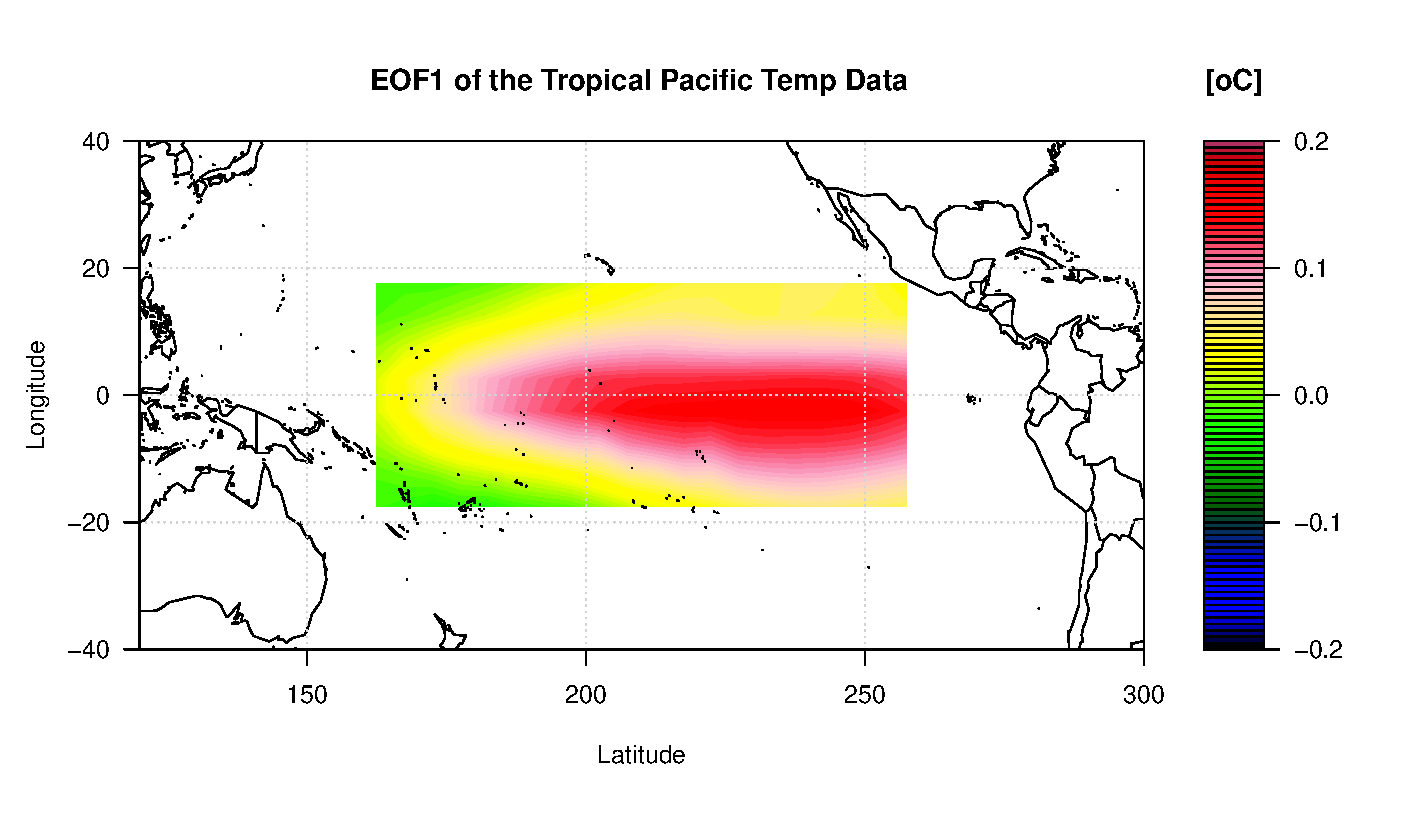
\includegraphics[height = 8cm]{Photos/EOF1}

			\newpage
\begin{Shaded}
\begin{Highlighting}[]
\NormalTok{umat =}\StringTok{ }\KeywordTok{matrix}\NormalTok{(U[,}\DecValTok{2}\NormalTok{], }\DataTypeTok{nrow =}\NormalTok{ numLonVals)}
\KeywordTok{filled.contour}\NormalTok{(y, x, umat, }\DataTypeTok{color.palette=}\NormalTok{rgb.palette, }\DataTypeTok{levels=}\NormalTok{int,}
               \DataTypeTok{xlim=}\KeywordTok{c}\NormalTok{(}\DecValTok{120}\NormalTok{,}\DecValTok{300}\NormalTok{),}\DataTypeTok{ylim=}\KeywordTok{c}\NormalTok{(}\OperatorTok{-}\DecValTok{40}\NormalTok{,}\DecValTok{40}\NormalTok{),}
               \DataTypeTok{plot.title=}\KeywordTok{title}\NormalTok{(}\DataTypeTok{main=}\StringTok{"EOF2 of the Tropical Pacific Temp Data"}\NormalTok{,}
                                \DataTypeTok{xlab=}\StringTok{"Latitude"}\NormalTok{,}\DataTypeTok{ylab=}\StringTok{"Longitude"}\NormalTok{),}
               \DataTypeTok{plot.axes=}\NormalTok{\{}\KeywordTok{axis}\NormalTok{(}\DecValTok{1}\NormalTok{); }\KeywordTok{axis}\NormalTok{(}\DecValTok{2}\NormalTok{); }\KeywordTok{map}\NormalTok{(}\StringTok{'world2'}\NormalTok{, }\DataTypeTok{add=}\OtherTok{TRUE}\NormalTok{); }\KeywordTok{grid}\NormalTok{()\},}
               \DataTypeTok{key.title=}\KeywordTok{title}\NormalTok{(}\DataTypeTok{main=}\StringTok{"[oC]"}\NormalTok{))}
\end{Highlighting}
\end{Shaded}
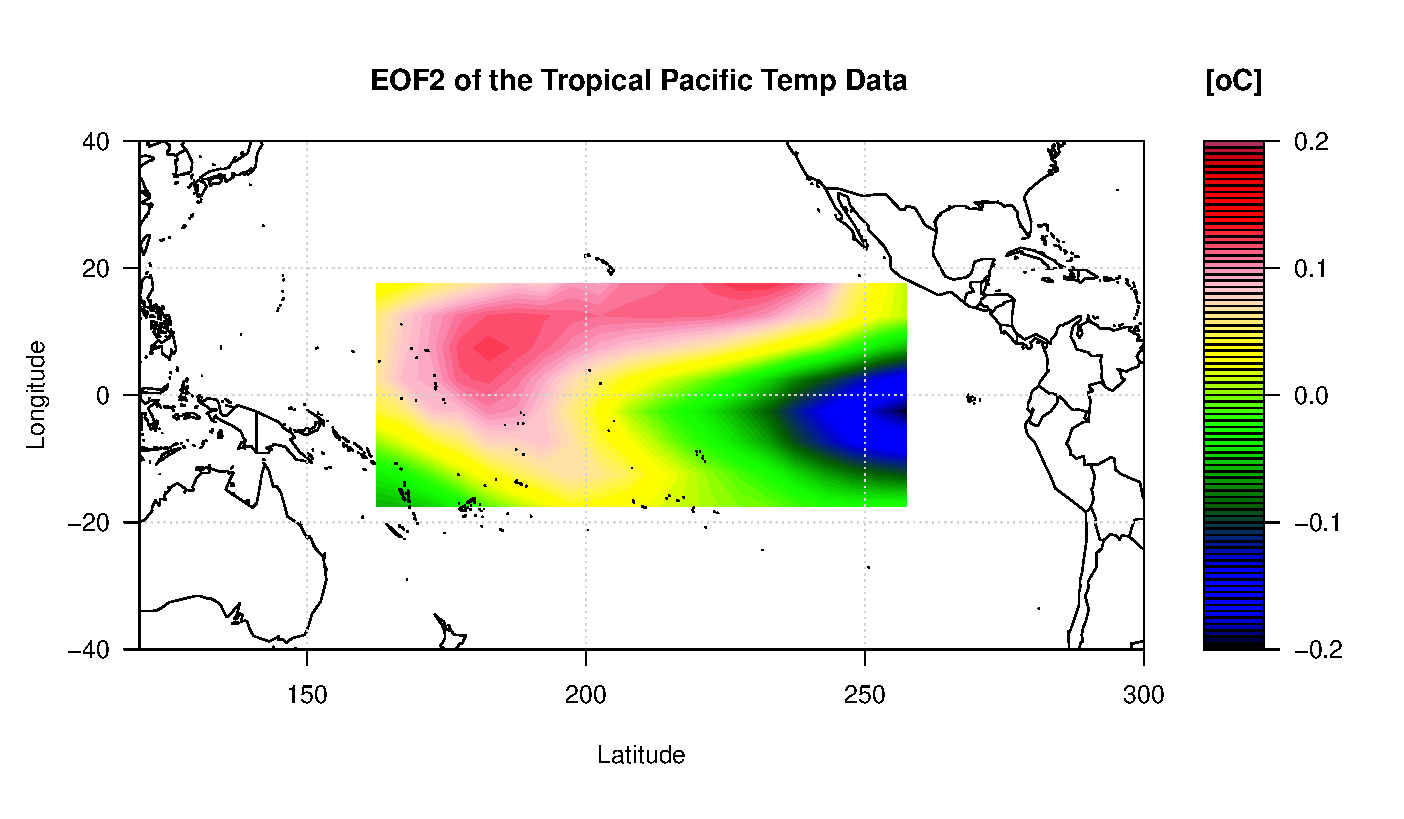
\includegraphics[height = 7.5cm]{Photos/EOF2}
\begin{Shaded}
\begin{Highlighting}[]
\NormalTok{umat =}\StringTok{ }\KeywordTok{matrix}\NormalTok{(U[,}\DecValTok{3}\NormalTok{], }\DataTypeTok{nrow =}\NormalTok{ numLonVals)}
\KeywordTok{filled.contour}\NormalTok{(y, x, umat, }\DataTypeTok{color.palette=}\NormalTok{rgb.palette, }\DataTypeTok{levels=}\NormalTok{int,}
               \DataTypeTok{xlim=}\KeywordTok{c}\NormalTok{(}\DecValTok{120}\NormalTok{,}\DecValTok{300}\NormalTok{),}\DataTypeTok{ylim=}\KeywordTok{c}\NormalTok{(}\OperatorTok{-}\DecValTok{40}\NormalTok{,}\DecValTok{40}\NormalTok{),}
               \DataTypeTok{plot.title=}\KeywordTok{title}\NormalTok{(}\DataTypeTok{main=}\StringTok{"EOF3 of the Tropical Pacific Temp Data"}\NormalTok{,}
                                \DataTypeTok{xlab=}\StringTok{"Latitude"}\NormalTok{,}\DataTypeTok{ylab=}\StringTok{"Longitude"}\NormalTok{),}
               \DataTypeTok{plot.axes=}\NormalTok{\{}\KeywordTok{axis}\NormalTok{(}\DecValTok{1}\NormalTok{); }\KeywordTok{axis}\NormalTok{(}\DecValTok{2}\NormalTok{); }\KeywordTok{map}\NormalTok{(}\StringTok{'world2'}\NormalTok{, }\DataTypeTok{add=}\OtherTok{TRUE}\NormalTok{); }\KeywordTok{grid}\NormalTok{()\},}
               \DataTypeTok{key.title=}\KeywordTok{title}\NormalTok{(}\DataTypeTok{main=}\StringTok{"[oC]"}\NormalTok{))}
\end{Highlighting}
\end{Shaded}
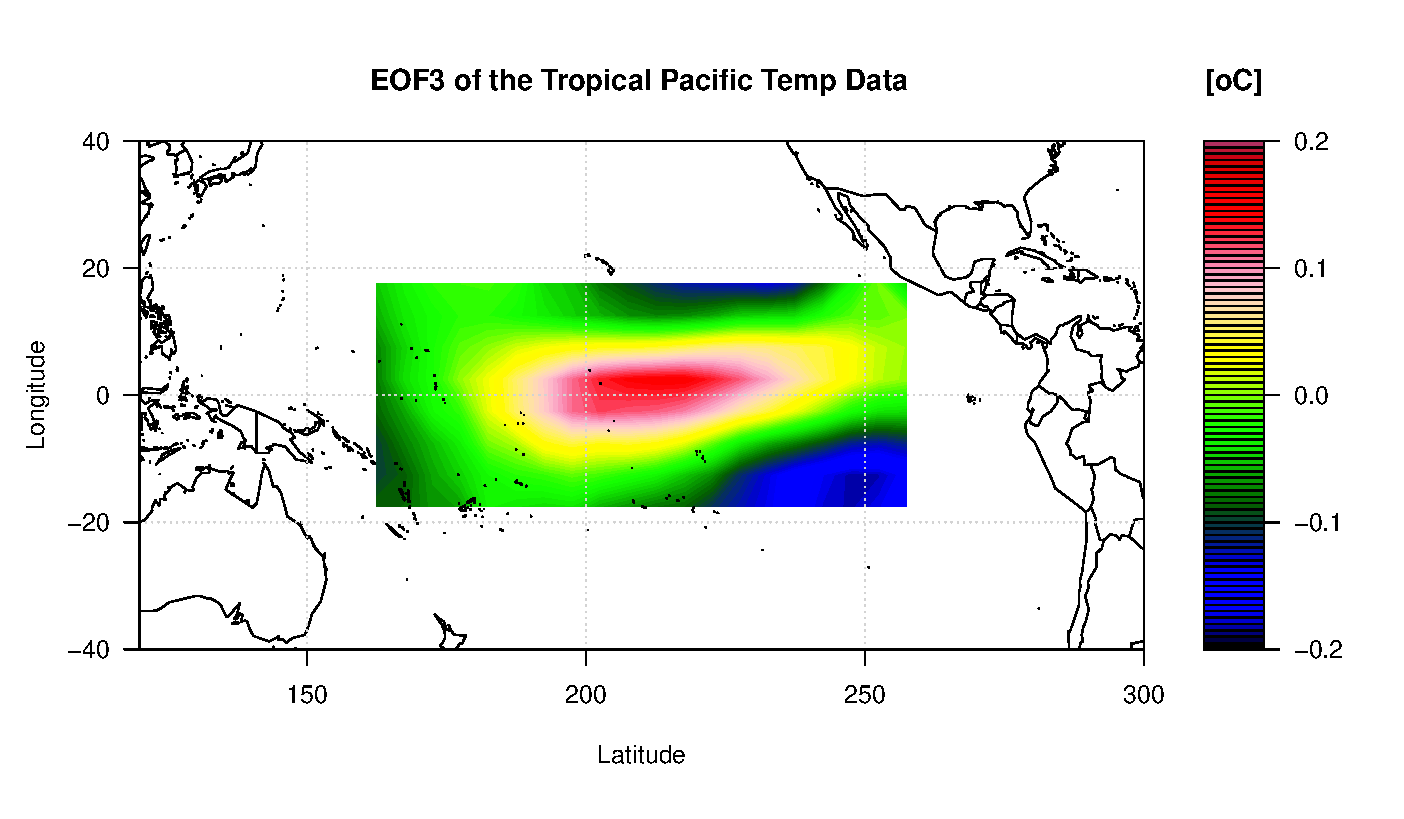
\includegraphics[height = 7.5cm]{Photos/EOF3}

			\item Plot the time series of the first three V column vectors, which are the temporal patterns
			of the data field, and are also known as Principal Components (PCs).
			
\begin{Shaded}
\begin{Highlighting}[]
\KeywordTok{plot}\NormalTok{(time, V[,}\DecValTok{1}\NormalTok{], }\StringTok{'l'}\NormalTok{, }\DataTypeTok{col =} \StringTok{'black'}\NormalTok{,}
     \DataTypeTok{xlab =} \StringTok{'Year'}\NormalTok{, }\DataTypeTok{ylab =} \StringTok{'PC Scale'}\NormalTok{, }\DataTypeTok{ylim=}\KeywordTok{c}\NormalTok{(}\OperatorTok{-}\FloatTok{0.4}\NormalTok{,}\FloatTok{0.4}\NormalTok{), }
\DataTypeTok{main =} \StringTok{'The First Three PCs'}\NormalTok{, }\DataTypeTok{panel.first=}\KeywordTok{grid}\NormalTok{())}
\KeywordTok{lines}\NormalTok{(time, V[,}\DecValTok{2}\NormalTok{], }\DataTypeTok{type=}\StringTok{"l"}\NormalTok{, }\DataTypeTok{col=}\StringTok{"blue"}\NormalTok{)}
\KeywordTok{lines}\NormalTok{(time, V[,}\DecValTok{3}\NormalTok{], }\DataTypeTok{type=}\StringTok{"l"}\NormalTok{, }\DataTypeTok{col=}\StringTok{"red"}\NormalTok{)}


\KeywordTok{legend}\NormalTok{(}\DecValTok{1950}\NormalTok{,}\FloatTok{0.4325}\NormalTok{, }\StringTok{'PC1'}\NormalTok{,}\DataTypeTok{lwd=}\DecValTok{2}\NormalTok{ )}
\KeywordTok{legend}\NormalTok{(}\DecValTok{1960}\NormalTok{,}\FloatTok{0.4325}\NormalTok{, }\StringTok{'PC2'}\NormalTok{,}\DataTypeTok{lwd=}\DecValTok{2}\NormalTok{, }\DataTypeTok{col=}\StringTok{"blue"}\NormalTok{)}
\KeywordTok{legend}\NormalTok{(}\DecValTok{1970}\NormalTok{,}\FloatTok{0.4325}\NormalTok{, }\StringTok{'PC3'}\NormalTok{,}\DataTypeTok{lwd=}\DecValTok{2}\NormalTok{, }\DataTypeTok{col=}\StringTok{"red"}\NormalTok{)}
\end{Highlighting}
\end{Shaded}

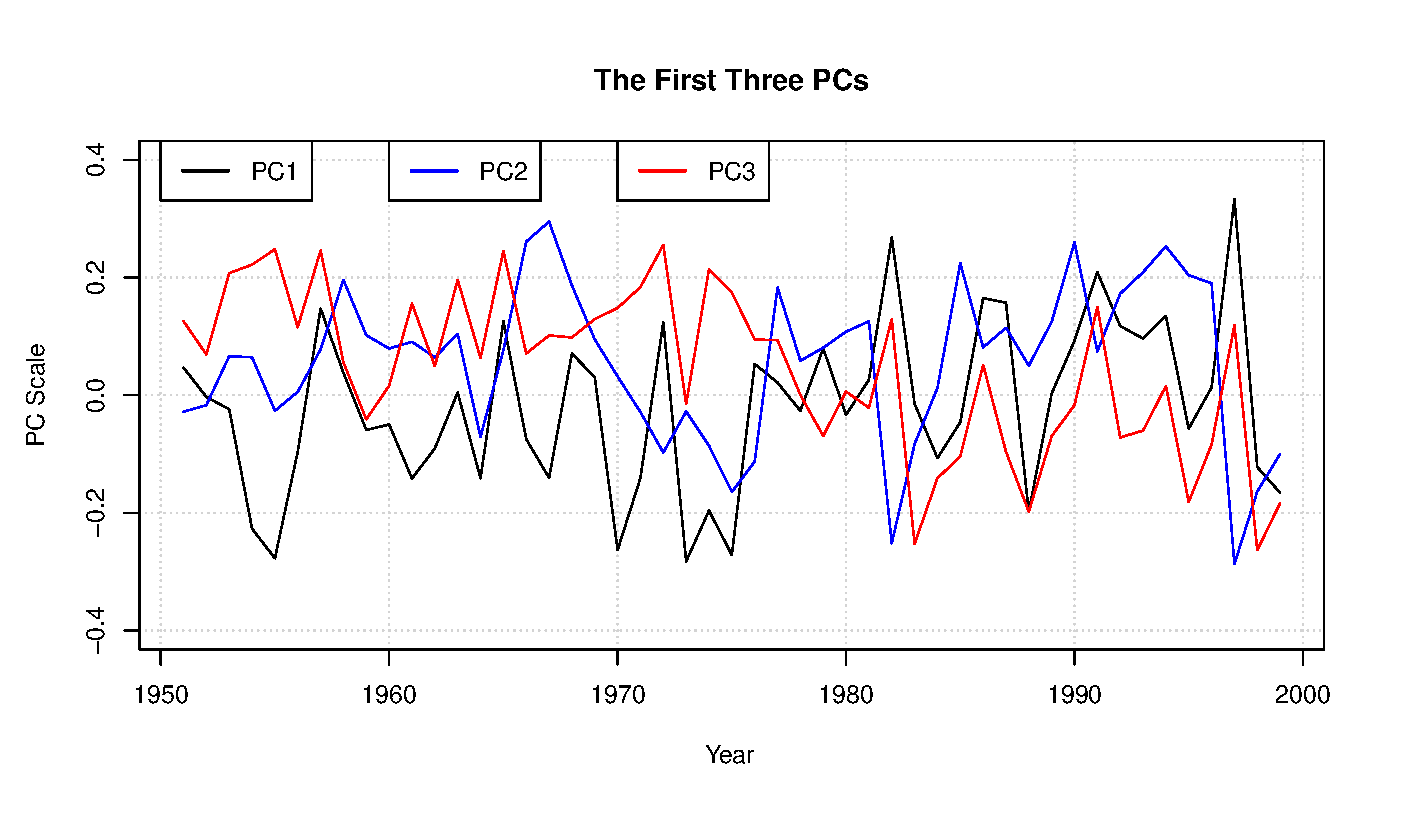
\includegraphics{Photos/PC}

			\item  El Nino signals should show in the figures of Steps (b) and (c). Make a brief description of the El Ninos.
			\\ \\
			You can see from the EOF's and PC's that the temperature spikes in the same location and the same time in the pacific ocean consistently.  These spikes are consistent with the data that we have on the El Ninos.  The El Ninos spike in temperature in the pacific ocean at $200^\circ$ Latitude on the equator and around the summer time.  During these El Ninos as well, we can see that the wind reverses to become western winds instead of eastern winds.
			
		\end{enumerate}
		
	\end{problem}

\end{document}
